% Allotrope - AIGC Stage-III evaluation committee, 2026-11-04 09:00. Deck v2: 15 main slides + 6 appendix.
% Consistent with the submitted report (PS11_stage3_report_allotrope21labs.pdf, 2 Nov 2026): numbers, story, terms.
% Sources sit in %% src: comments ("R p.N" = report page N); NUMBERS.md lists them.
% No source file, code identifier or commit on any slide (user rule).
% Build: PYTHONPATH=C:/pdfr C:/av/Scripts/python.exe make_figures.py, then C:/Users/FITT/tools/tectonic/tectonic.exe main.tex,
% then PYTHONPATH=C:/pdfr C:/av/Scripts/python.exe render_pages.py
\documentclass[aspectratio=169,10pt]{beamer}
% Allotrope v1.0 deck theme: quiet, Tufte-like, matching the product's v1.0 UI.
% Paper #fffff8, ink #111, hairlines #ddd; man-made #c0392b, natural #2e7d6b, anomaly/selection ochre #d4a017.
\usepackage{fontspec}
\usepackage{unicode-math}
\setmainfont{texgyrepagella}[Extension=.otf, UprightFont=*-regular, BoldFont=*-bold,
  ItalicFont=*-italic, BoldItalicFont=*-bolditalic, Numbers={Lining,Monospaced}]
\setsansfont{texgyrepagella}[Extension=.otf, UprightFont=*-regular, BoldFont=*-bold,
  ItalicFont=*-italic, BoldItalicFont=*-bolditalic, Numbers={Lining,Monospaced}]
\setmonofont{texgyrecursor}[Extension=.otf, UprightFont=*-regular, BoldFont=*-bold, Scale=0.95]
\setmathfont{texgyrepagella-math.otf}
\usefonttheme{professionalfonts}
\usefonttheme{serif}

\usepackage{booktabs,array,tabularx,colortbl,multirow,makecell}
\usepackage{tikz,pgfplots}
\usetikzlibrary{arrows.meta,positioning,calc,decorations.pathreplacing,shapes.misc}
\pgfplotsset{compat=1.18}
\usepgfplotslibrary{groupplots}

\definecolor{paper}{HTML}{FFFFF8}
\definecolor{ink}{HTML}{111111}
\definecolor{rule}{HTML}{DDDDDD}
\definecolor{mute}{HTML}{6B6B6B}
\definecolor{faint}{HTML}{A8A8A8}
\definecolor{manmade}{HTML}{C0392B}
\definecolor{natural}{HTML}{2E7D6B}
\definecolor{ochre}{HTML}{D4A017}
\definecolor{band}{HTML}{F4F1E6}

\setbeamercolor{background canvas}{bg=paper}
\setbeamercolor{normal text}{fg=ink,bg=paper}
\setbeamercolor{structure}{fg=ink}
\setbeamercolor{alerted text}{fg=manmade}
\setbeamercolor{frametitle}{fg=ink}
\setbeamercolor{block title}{fg=ink,bg=}
\setbeamercolor{block body}{fg=ink,bg=}
\setbeamertemplate{navigation symbols}{}
\setbeamertemplate{blocks}[default]
\setbeamersize{text margin left=6mm, text margin right=6mm}

\setbeamertemplate{frametitle}{%
  \vspace*{2.2mm}{\fontsize{12.5}{14.5}\selectfont\insertframetitle\par}%
  \vspace{0.8mm}{\color{rule}\rule{\textwidth}{0.4pt}}\vspace{-1mm}}

\newcommand{\decklabel}{Allotrope v1.0 \textperiodcentered{} AIGC Stage III}
% Allotrope21 Labs mark (octahedron), redrawn as a vector in ink for the paper background. #1 = half-height.
\newcommand{\alogomark}[2][ink]{\tikz[baseline=-0.6ex, x=#2, y=#2, line cap=round, line join=round]{%
  \draw[#1, line width=0.06*#2] (0,1) -- (-0.62,0) -- (0,-1) -- (0.62,0) -- cycle (0,1) -- (0,-1);
  \draw[#1, line width=0.04*#2, dash pattern=on 0.07*#2 off 0.07*#2] (0,0) ellipse [x radius=0.62, y radius=0.13];
  \foreach \p in {(0,1),(0,-1),(-0.62,0),(0.62,0)} \fill[#1] \p circle (0.075);
  \foreach \p in {(0,0.32),(0,-0.32)} \fill[#1] \p circle (0.05);}}
% Mark + wordmark: ALLOTROPE 21 in ink, LABS in grey.
\newcommand{\alogo}[2]{\alogomark{#1}\hspace{0.55em}{#2\addfontfeatures{LetterSpace=6}ALLOTROPE\,21\hspace{0.45em}{\color{faint}LABS}}}
\setbeamertemplate{footline}{%
  \hbox to \paperwidth{\hspace{6mm}{\color{mute}\alogo{1.15ex}{\fontsize{5.6}{7}\selectfont}\hspace{1.2em}\fontsize{6.5}{8}\selectfont\decklabel}\hfill
  {\color{mute}\fontsize{6.5}{8}\selectfont\insertframenumber}\hspace{6mm}}\vspace{2.2mm}}

\setbeamertemplate{itemize item}{\raisebox{0.25ex}{\color{ochre}\rule{0.5ex}{0.5ex}}}
\setbeamertemplate{itemize subitem}{\color{mute}--}
\setlength{\leftmargini}{1.0em}
\setbeamerfont{itemize/enumerate body}{size=\small}
\setbeamerfont{itemize/enumerate subbody}{size=\footnotesize}

\renewcommand{\arraystretch}{1.08}
\setlength{\tabcolsep}{3pt}
\arrayrulecolor{faint}
\setlength{\heavyrulewidth}{0.5pt}\setlength{\lightrulewidth}{0.3pt}\setlength{\cmidrulewidth}{0.3pt}

% small helpers
\newcommand{\sfr}[1]{\includegraphics[width=20.6mm]{figures/story_prisma_k#1.jpg}}  % story frame
\newcommand{\src}[1]{{\color{mute}\fontsize{5.6}{6.6}\selectfont #1\par}}
\newcommand{\srcc}[1]{{\color{mute}\fontsize{5.6}{6.6}\selectfont #1}}       % on-slide source note
\newcommand{\kicker}[1]{{\color{mute}\scriptsize\scshape #1}}                 % panel heading
\newcommand{\hl}[1]{\textbf{#1}}
\newcommand{\mm}{{\color{manmade}man-made}}
\newcommand{\nat}{{\color{natural}natural}}
\newcommand{\shp}[1]{{\ttfamily\fontsize{5.4}{6}\selectfont #1}}             % tensor shape on arrows
\newcommand{\fn}[1]{{\ttfamily\fontsize{6.3}{7.4}\selectfont #1}}             % file name

\pgfplotsset{tufte/.style={
  axis line style={draw=none}, tick style={draw=none},
  ticklabel style={font=\fontsize{6.5}{7}\selectfont, color=mute},
  label style={font=\fontsize{6.5}{7}\selectfont, color=mute},
  grid=none, every axis plot/.append style={line join=round}}}

\tikzset{blk/.style={draw=ink, line width=0.4pt, align=center, inner sep=2pt,
    font=\fontsize{6.4}{7.4}\selectfont, fill=paper},
  arr/.style={-{Stealth[length=1.6mm,width=1.2mm]}, line width=0.45pt, draw=ink}}
\tikzset{ms/.style={font=\fontsize{5.9}{6.9}\selectfont, align=left, anchor=south west, inner sep=0.5pt, text width=#1}}
\tikzset{fl/.style={font=\fontsize{5.7}{6.7}\selectfont, align=left, anchor=north west, inner sep=0.5pt, text width=#1, color=manmade!85!ink}}
\usepackage{adjustbox}
\newcommand{\fitw}[1]{\adjustbox{max width=\linewidth}{#1}}
\usetikzlibrary{patterns,fit,backgrounds,shapes.geometric}
\definecolor{pY}{HTML}{F6E7A1}\definecolor{pB}{HTML}{CFE0F3}\definecolor{pG}{HTML}{D4EAD6}\definecolor{pR}{HTML}{F2C4BC}
% NAS-figure style: dashed tinted group containers, hatched stage blocks, pastel cells, open loss circles
\tikzset{
  grp/.style={draw=mute, dashed, rounded corners=3pt, line width=0.5pt, inner sep=2mm},
  stg/.style={draw=ink!70, rounded corners=1.5pt, line width=0.5pt, preaction={fill=paper},
    pattern=north east lines, pattern color=ochre!45, align=center, font=\itshape\fontsize{6.4}{7.4}\selectfont, inner sep=1pt},
  stgn/.style={stg, draw=ochre!85!black, line width=0.9pt},
  stgx/.style={stg, draw=faint, pattern color=faint!30, text=mute},
  cell/.style={draw=ink!50, line width=0.3pt, minimum size=1.9mm, inner sep=0pt},
  loss/.style={draw=ochre!90!black, line width=0.6pt, ellipse, inner sep=0.8pt, font=\itshape\fontsize{5.8}{6.6}\selectfont, fill=paper},
  glab/.style={font=\itshape\fontsize{6.6}{7.6}\selectfont, color=ink!80, anchor=north west, inner sep=1pt, xshift=1.2mm, yshift=-1mm},
  tsh/.style={font=\itshape\fontsize{5.4}{6}\selectfont, color=mute},
  df/.style={-{Stealth[length=1.5mm,width=1.1mm]}, line width=0.5pt, draw=ink},
  tf/.style={-{Stealth[length=1.5mm,width=1.1mm]}, line width=0.5pt, draw=mute, dashed}}
\newcommand{\take}[1]{\par\vspace{0.6mm}{\color{ink}\fontsize{7.2}{8.6}\selectfont\itshape #1\par}}

\title{Allotrope}
\date{4 November 2026}
\renewcommand{\decklabel}{AIGC Stage III}
\newcommand{\eqs}[1]{{\fontsize{7.6}{9.4}\selectfont #1\par}}
\newcommand{\tx}[1]{{\fontsize{6.6}{7.9}\selectfont #1\par}}

\begin{document}

%======================================================================
% 1 TITLE
%======================================================================
\begin{frame}[plain]
\begin{columns}[T,onlytextwidth]
\column{0.56\textwidth}
\vspace*{1mm}
{\alogo{2.2ex}{\fontsize{9}{11}\selectfont}\par}
\vspace{2mm}
{\fontsize{26}{28}\selectfont Allotrope\par}
\vspace{1.5mm}
{\fontsize{12.5}{15}\selectfont Anomaly detection, material identification\\ and atmospheric correction\\ in hyperspectral satellite imagery\par}
\vspace{3mm}
{\color{rule}\rule{0.9\linewidth}{0.4pt}}\par\vspace{1.5mm}
{\small Indradhanu, our own spectral foundation model, learns ordinary ground; what it cannot rebuild is flagged, then named \mm{} or \nat{} with its closest material class.\par}
\vspace{4mm}
{\footnotesize AIGC Stage-III evaluation \textperiodcentered{} PS-11\\
4 November 2026, 09:00\par}
\vspace{5mm}
\fitw{\begin{tabular}{@{}lll@{}}
\toprule
{\fontsize{16}{18}\selectfont 0.189} & {\fontsize{16}{18}\selectfont 449\,/\,909} & {\fontsize{16}{18}\selectfont 86--94\,\%}\\
\scriptsize pAUC, false alarms $\le$1\,\% & \scriptsize objects in the top 1\,\% & \scriptsize \mm{} targets found\\
\scriptsize previous release 0.170 & \scriptsize no model 377 & \scriptsize at quarter-pixel fill; ACE 66--77\,\%\\
\bottomrule
\end{tabular}}
%% src: R p.1 summary (0.189 vs 0.170; 449, 418, 377, 93; 86-94 % vs 66-77 %)
\column{0.42\textwidth}
\vspace*{4mm}
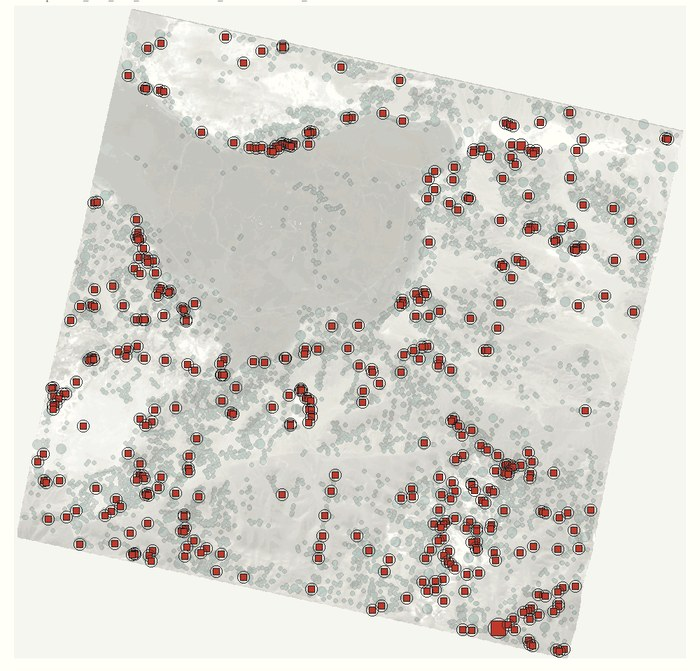
\includegraphics[width=\linewidth]{figures/story_prisma_k7.jpg}\par
\src{PRISMA, 14 Feb 2025: 405 of 5,544 anomaly objects called man-made.}
%% src: R p.2 Figure 1 caption (5,544 objects, 405 man-made)
\end{columns}
\end{frame}

%======================================================================
% 2 PROBLEM AND DATA
%======================================================================
\begin{frame}{Problem and data}
\begin{columns}[T,onlytextwidth]
\column{0.50\textwidth}
\kicker{the task}\par\vspace{0.3mm}
\tx{Find small, unusual objects in hyperspectral images with no target list given in advance, and say what material each is made of. At Stage II our model (700+ scenes) raised false alarms on urban scenes, land--water edges, cloud contours and snow; Stage III widened the data and moved the model's attention to the spectrum.}
%% src: R p.1 Introduction
\vspace{1.6mm}
\kicker{data procured for Stage III}\par\vspace{0.3mm}
\fitw{\fontsize{6.6}{7.9}\selectfont\begin{tabular}{@{}lp{50mm}@{}}
\toprule
pretraining & SpectralEarth, all of it: $\approx$3.3\,TB, $\approx$11,636 EnMAP scenes, 539,755 patches\\
curated & 1,300+ EnMAP, PRISMA and AVIRIS-NG scenes; India and borders; urban, forest, desert, hills, coast; 2--40\,\% cloud\\
L1 / L2 pairs & 60 EnMAP and 30 PRISMA (L1, L2C, L2D) for atmospheric correction; 50+ public Tanager scenes\\
\bottomrule
\end{tabular}}\par
%% src: R p.1-2 Section 1; R p.4 (539,755); R p.18 (60 / 30 pairs, 50+ Tanager)
\vspace{1.6mm}
\kicker{sensors}\par\vspace{0.3mm}
\fitw{\fontsize{6.6}{7.9}\selectfont\begin{tabular}{@{}llll@{}}
\toprule
sensor & bands in the file & pixel & role\\
\midrule
PRISMA & 239 (185 used) & 30\,m & test bench; fine-tuning; namer\\
EnMAP & 224 & 30\,m & pretraining; fine-tuning; namer\\
AVIRIS-NG & 372 & varies & fine-tuning; namer; field targets\\
Tanager & 426 (368 good) & 30\,m & end to end; never trained on\\
\bottomrule
\end{tabular}}\par
%% src: R p.2 Table 1
\column{0.46\textwidth}
\kicker{the test bench}\par\vspace{0.3mm}
\tx{Four labelled PRISMA L2D scenes, \textbf{909 ground-truth objects} in three tiers (easy, medium, subtle). Every method is scored on the same valid pixels and the same object maps.}
%% src: R p.2
\vspace{1.6mm}
\kicker{measures}\par\vspace{0.3mm}
\fitw{\fontsize{6.6}{7.9}\selectfont\begin{tabular}{@{}l>{\raggedright}p{38mm}l@{}}
\toprule
measure & what it means & chance\\
\midrule
\textbf{pAUC} & area under the detection curve while false alarms stay $\le$1\,\% of background, scaled so 1 is perfect & $\approx$0.005\\
top 1\,\% & object found if any pixel lies within 1\,px of the top 1\,\% of scores & 10.2\,\% (93)\\
top 0.1\,\% & the same, ten times stricter & 1.1\,\%\\
ROC-AUC & ranking over all thresholds & 0.5\\
bootstrap & resample the 909 objects 2,000 times; 95\,\% interval of the difference & \\
\bottomrule
\end{tabular}}\par
%% src: R p.2 Table 2
\vspace{1mm}
\src{Bench resolution: about $\pm$0.005--0.01 pAUC.}
\end{columns}
\end{frame}

%======================================================================
% 3 PIPELINE
%======================================================================
\begin{frame}{Pipeline}
\centering
\resizebox{\textwidth}{!}{%
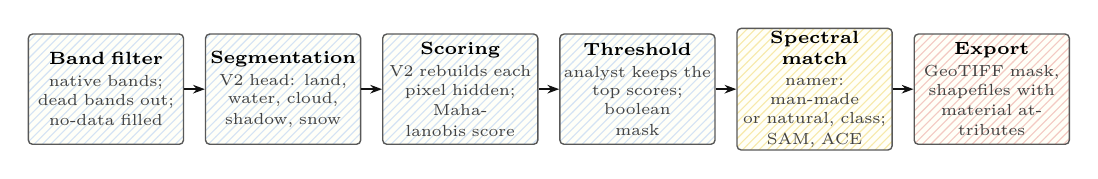
\begin{tikzpicture}[x=1mm,y=1mm]
\foreach \i/\t/\b/\c in {
 {0/Band filter/native bands;\\dead bands out;\\no-data filled/pB},
 {1/Segmentation/V2 head: land,\\water, cloud,\\shadow, snow/pB},
 {2/Scoring/V2 rebuilds each\\pixel hidden;\\Mahalanobis score/pB},
 {3/Threshold/analyst keeps the\\top scores; boolean\\mask/pB},
 {4/Spectral match/namer: man-made\\or natural, class;\\SAM, ACE/pY},
 {5/Export/GeoTIFF mask,\\shapefiles with\\material attributes/pR}}{
  \node[stg, pattern color=\c!90, minimum width=19mm, minimum height=14mm, text width=19mm] (n\i) at (\i*22.5, 0)
    {\textbf{\upshape\t}\\[0.4mm]{\upshape\color{ink!80}\fontsize{5.8}{6.8}\selectfont \b}};}
\foreach \i [evaluate=\i as \j using int(\i+1)] in {0,...,4} \draw[df] (n\i.east) -- (n\j.west);
\end{tikzpicture}}
%% src: R p.2 Figure 1 and text; R p.17 (ATM); R p.16 (deliverables)
\vspace{1.2mm}
\begin{columns}[T,onlytextwidth]
\column{0.68\textwidth}
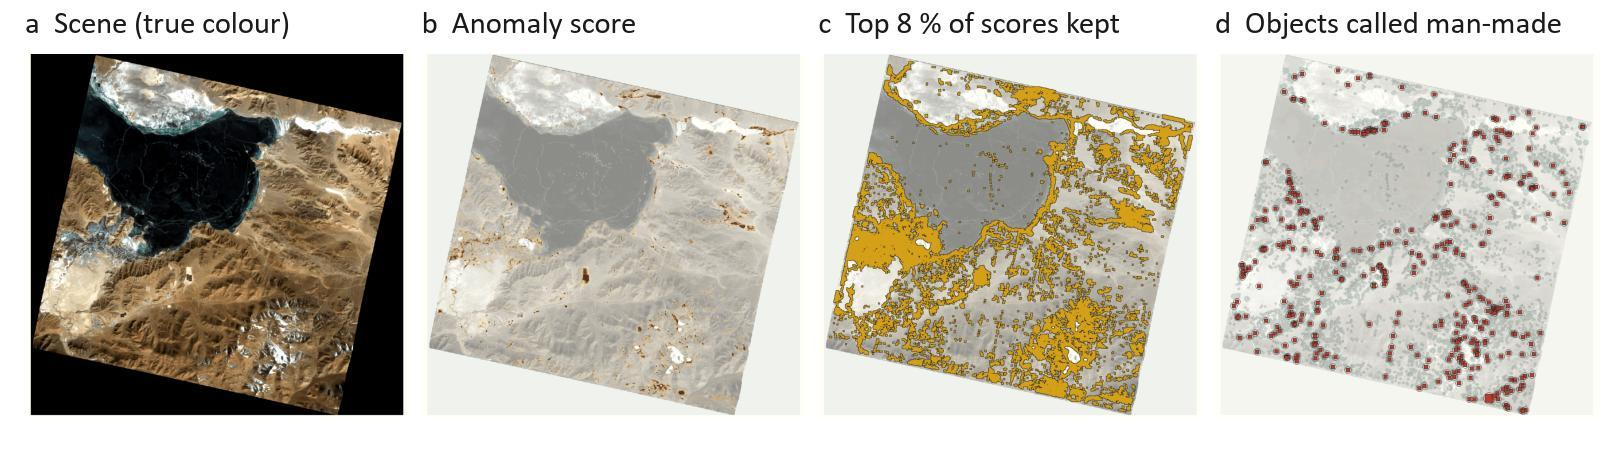
\includegraphics[width=\linewidth]{figures/rep_fig1_chain.jpg}\par
\src{One PRISMA scene (14 Feb 2025, 1237$\times$1202 px) through the chain: 30.3\,\% no-data; thick cloud (4.9\,\%) left out; the analyst keeps the top 8\,\%, 118,950 pixels; 5,544 objects named, 405 \mm{} (red).}
%% src: R p.2 Figure 1 caption
\column{0.29\textwidth}
\kicker{time per PRISMA scene}\par\vspace{0.3mm}
\fitw{\fontsize{6.6}{7.9}\selectfont\begin{tabular}{@{}lr@{}}
\toprule
V2 Heavy, 16-thread CPU & 454 s\\
\quad previous release & 274 s\\
residual Mahalanobis & 3--4 s\\
spectral namer & 8--9 s\\
\bottomrule
\end{tabular}}\par
%% src: R p.20 (PRISMA 13 min on the VM); R p.15 (454 vs 274 s); R p.3 (3-4 s); R p.9 (8-9 s)
\vspace{1.2mm}
\tx{The matcher's \nat{} call removes natural anomalies after scoring, with a tunable confidence.}
%% src: R p.2 ("filtering out natural anomalies ... tunable confidence")
\end{columns}
\end{frame}

%======================================================================
% 4 SPATIAL TO SPECTRAL
%======================================================================
\begin{frame}{Spatial to spectral}
\centering
% Indradhanu V1 (v0.2.0) against V2 (Heavy, v2.1.0), in the grouped/hatched style; V2's new parts outlined in ochre.
% Sources: docs/04-models.md (V1: 165-band grid, 1x1 compressor to 24-32 channels, SegFormer MAE, pixel-shuffle decoder, 5.5 M;
% V2: wavelength stem, [96,192,480,768], heads [3,6,10,12], progressive decoder 512 -> 256/128, 35.3 M);
% docs/lld/spectral-stem.md (40 nm bins, per-band skip, thick-cloud rule); research/textbook/chapters/41-heavy.tex (33,884,194 + 1,431,120).
\adjustbox{max width=\textwidth, max totalheight=0.53\textheight}{%
\begin{tikzpicture}[x=1mm,y=1mm]
% ---------------- V1 ----------------
\node[grp, fill=pB!35, minimum width=176mm, minimum height=24mm, anchor=north west] (G1) at (0,0) {};
\node[glab] at (G1.north west) {Indradhanu V1 (v0.2.0) \textperiodcentered{} 5.5\,M parameters \textperiodcentered{} a spatial model: 165 resampled bands are fixed input channels};
\node[inner sep=0, anchor=west] (i1) at (4,-13) {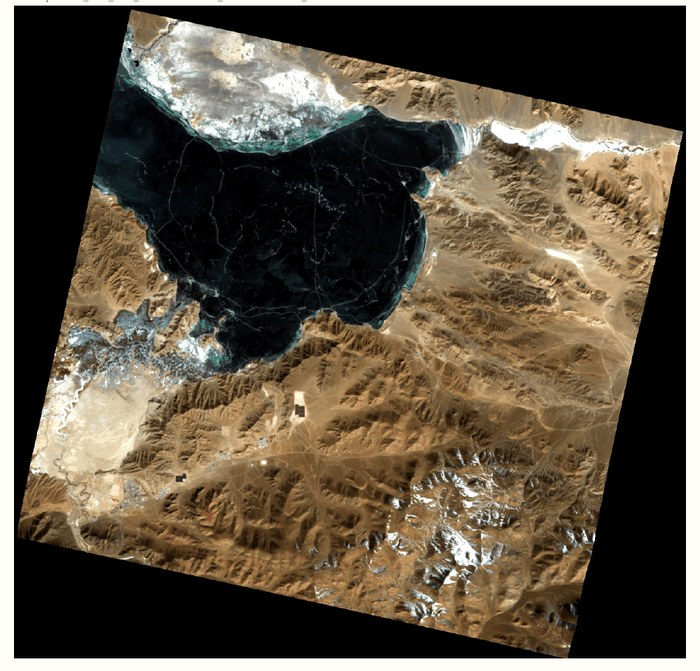
\includegraphics[width=12mm]{figures/story_prisma_k1.jpg}};
\node[tsh, below=0.3mm of i1] {165-band grid};
\node[stg, minimum width=15mm, minimum height=10mm] (c1) at (31,-13) {1$\times$1\\compressor};
\node[tsh, above=0.4mm of c1] {165 $\to$ 24--32 ch};
\node[grp, fill=pG!30, minimum width=58mm, minimum height=17mm] (E1) at (75,-13.5) {};
\node[glab] at (E1.north west) {Encoder};
\foreach \i/\x in {1/53,2/67,3/81,4/95} {
  \node[stg, minimum width=11mm, minimum height=9mm] (s1\i) at (\x,-14.5) {};
  \node[font=\itshape\fontsize{6}{7}\selectfont] at (\x,-12.2) {stage \i};
  \node[cell, fill=pG] at (\x-1.4,-16.4) {}; \node[cell, fill=pG] at (\x+1.4,-16.4) {};}
\foreach \i [evaluate=\i as \j using int(\i+1)] in {1,2,3} \draw[df] (s1\i) -- (s1\j);
\node[grp, fill=pY!35, minimum width=20mm, minimum height=17mm] (D1) at (120,-13.5) {};
\node[glab] at (D1.north west) {Decoder};
\node[stg, minimum width=14mm, minimum height=9mm] (d1) at (120,-14.5) {SegFormer\\pixel shuffle};
\node[font=\fontsize{7}{8}\selectfont] (o1) at (143,-13) {$\hat{\mathbf x}$};
\node[loss] (l1) at (156,-8) {L1 + SAM};
\node[loss] (r1) at (156,-18) {combined score};
\draw[df] (i1) -- (c1); \draw[df] (c1) -- (s11); \draw[df] (s14) -- (d1); \draw[df] (d1) -- (o1);
\draw[tf] (o1) -- (l1); \draw[df] (o1) -- (r1);
% ---------------- V2 ----------------
\node[grp, fill=pR!30, minimum width=176mm, minimum height=40mm, anchor=north west] (G2) at (0,-28) {};
\node[glab] at (G2.north west) {Indradhanu V2 (v2.1.0, Heavy) \textperiodcentered{} 33.9\,M + 1.43\,M head = 35.3\,M parameters \textperiodcentered{} spectral: bands enter as (value, wavelength)};
\node[inner sep=0, anchor=west] (i2) at (4,-46) {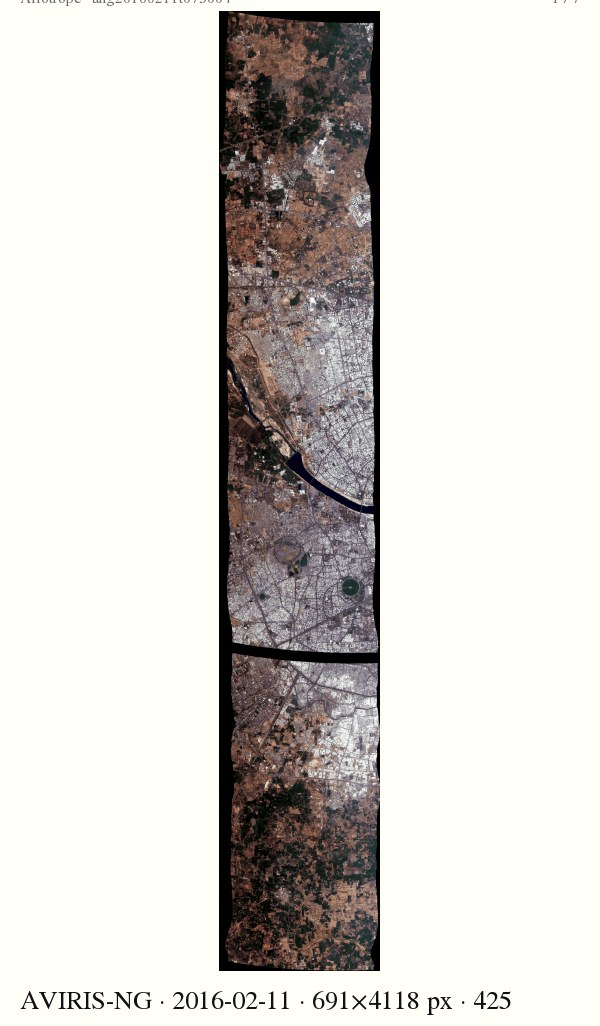
\includegraphics[width=12mm]{figures/story_aviris_k1.jpg}};
\draw[ochre!85!black, line width=0.6pt] plot[smooth] coordinates {(4,-60) (6,-58.2) (8,-57.5) (9.5,-59.5) (11,-56.8) (13,-57.3) (16,-58.6)};
\node[tsh, text=ochre!80!black] at (10,-62.5) {any bands, native};
% stem
\node[grp, fill=pY!30, draw=ochre!85!black, solid, minimum width=30mm, minimum height=26mm] (S2) at (37,-47) {};
\node[glab] at (S2.north west) {Spectral stem};
\foreach \k in {0,...,6} \node[cell, fill=pY] at (26.5+\k*2.9,-42.4) {};
\node[tsh] at (35.2,-39.8) {40\,nm wavelength bins};
\foreach \k in {0,...,3} \node[cell, circle, fill=pB] at (30.8+\k*2.9,-47.5) {};
\node[tsh] at (35.2,-51) {attention, 4 heads};
\node[stgn, minimum width=13mm, minimum height=4.5mm] (z2) at (35.2,-56.4) {64 ch};
\draw[df] (35.2,-43.6) -- (35.2,-45.8); \draw[df] (35.2,-49.2) -- (z2);
% encoder
\node[grp, fill=pG!30, draw=ochre!85!black, solid, minimum width=62mm, minimum height=26mm] (E2) at (90,-47) {};
\node[glab] at (E2.north west) {Encoder, 3$\times$ wider};
\foreach \i/\x/\w/\c/\h in {1/68/8/96/3,2/80/10/192/6,3/94/12.5/480/10,4/110/15/768/12} {
  \node[stgn, minimum width=\w mm, minimum height=11mm] (s2\i) at (\x,-48) {};
  \node[font=\itshape\fontsize{6}{7}\selectfont] at (\x,-45.2) {stage \i};
  \node[cell, fill=pG] at (\x-1.4,-49) {}; \node[cell, fill=pG] at (\x+1.4,-49) {};
  \node[font=\itshape\fontsize{5.2}{6}\selectfont] at (\x,-51.6) {\c, \h\ h};}
\foreach \i [evaluate=\i as \j using int(\i+1)] in {1,2,3} \draw[df] (s2\i) -- (s2\j);
% decoder
\node[grp, fill=pY!30, draw=ochre!85!black, solid, minimum width=24mm, minimum height=26mm] (D2) at (138,-47) {};
\node[glab] at (D2.north west) {Decoder};
\node[stgn, minimum width=18mm, minimum height=5mm] (u1) at (138,-43.5) {fuse 512 $\to$ 256};
\node[stgn, minimum width=18mm, minimum height=5mm] (u2) at (138,-52.5) {up 256 $\to$ 128};
\draw[df] (u1) -- (u2);
% heads
\node[font=\fontsize{7}{8}\selectfont] (o2) at (158,-40) {$\hat{\mathbf x}$};
\node[loss] (l2) at (173,-36) {L1 + SAM};
\node[loss] (r2) at (173,-44.5) {Mahalanobis};
\node[stgn, minimum width=13mm, minimum height=7mm] (h2) at (164,-58) {seg head};
\node[tsh] at (164,-63.6) {land water cloud shadow snow};
\node[loss] (b2) at (176,-52) {BCE+Dice};
% flows
\draw[df] (i2) -- (S2.west |- i2); \draw[df] (z2.east) -- (s21.west |- z2.east) ;
\draw[df] (s24) -- (u1.west |- s24);
\draw[df] (u2.east) -| (o2.south);
\draw[tf] (o2) -- (l2); \draw[df] (o2) -- (r2);
\draw[tf, draw=ochre!85!black] (s24.north) -- (110,-31.5) -| (h2.north);
\draw[tf] (h2) -- (b2);
\draw[tf] (z2.south) -- ++(0,-6.5) -| node[pos=0.3, tsh, above]{skip at full resolution, hidden pixels zeroed} (u2.south);
% ---------------- legend ----------------
\begin{scope}[shift={(4,-75)}]
\node[stg, minimum width=7mm, minimum height=3.5mm] at (3,0) {}; \node[tsh, anchor=west, text=ink] at (7.5,0) {stage block};
\node[cell, fill=pG] at (30,0) {}; \node[cell, fill=pY] at (32.5,0) {}; \node[cell, circle, fill=pB] at (35,0) {}; \node[tsh, anchor=west, text=ink] at (37,0) {cells: transformer blocks, wavelength bins, attention heads};
\node[loss] at (101,0) {loss}; \node[tsh, anchor=west, text=ink] at (105,0) {loss / score};
\draw[df] (124,0) -- (131,0); \node[tsh, anchor=west, text=ink] at (132,0) {data flow};
\draw[tf] (147,0) -- (154,0); \node[tsh, anchor=west, text=ink] at (155,0) {training-only / optional};
\draw[ochre!85!black, line width=0.9pt, rounded corners=1pt] (-1,-4.5) rectangle (6,-2.6); \node[tsh, anchor=west, text=ink] at (7.5,-3.6) {new in V2};
\end{scope}
\end{tikzpicture}}

%% src: R p.3 Figure 2 and Section 2.1; R p.5 spec sheet; parameter counts research/textbook/chapters/41-heavy.tex
\vspace{0.6mm}
\begin{columns}[T,onlytextwidth]
\column{0.32\textwidth}
\kicker{V1, Stage II}\par\vspace{0.2mm}
\tx{A spatial SegFormer MAE on one resampled 165-band grid; a 1$\times$1 compressor ties weights to band position: it knows ``input 87'', not 1,650\,nm.}
\column{0.33\textwidth}
\kicker{V2, Stage III}\par\vspace{0.2mm}
\tx{A wavelength-aware stem turns each pixel into tokens over 40\,nm bins and attends over them: PRISMA's 185, EnMAP's 224, AVIRIS-NG's 372 bands read natively.}
\column{0.31\textwidth}
\kicker{what made it a foundation model}\par\vspace{0.2mm}
\tx{SpectralEarth pretraining (512,849 patches), band-subset and wavelength-jitter augmentation, 3$\times$ wider encoder, progressive decoder, segmentation head.}
\end{columns}
%% src: R p.3 bullets; docs/04-models.md (V1 1x1 compressor 165 -> 24-32 ch); spectral_tokens docstring ("input 87")
\take{pAUC 0.165 (V1) $\to$ 0.170 (V2.0) $\to$ 0.189 (V2 Heavy) on the 909-object bench, thick cloud excluded.}
%% src: R p.4 Table 3
\end{frame}

%======================================================================
% 5 SPECTRAL STEM
%======================================================================
\begin{frame}{Spectral stem}
\kicker{two real band lists, one token grid: every sensor's bands fall into the same 40\,nm bins}\par\vspace{0.1mm}
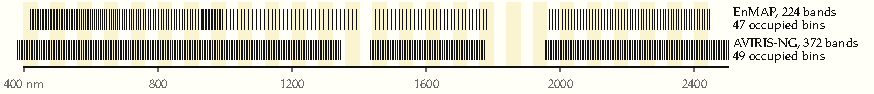
\includegraphics[width=\textwidth]{figures/chart_bands.pdf}\par
%% src: research/experiments/indradhanu-finetune/band_lists/enmap_224.json, aviris_ng_372.json (plotted); bins 40 nm from 400 nm (spectral stem source)
\vspace{0.6mm}
\begin{columns}[T,onlytextwidth]
\column{0.47\textwidth}
% The wavelength-binned spectral stem of Indradhanu V2 (reduced attention), NAS-figure style.
% Mechanism verified against app/foundation_models/components/spectral_reduced.py and spectral_tokens.py:
% 40 nm bins from 400 nm (53), bin token = width-weighted mean of x_b k(e(lambda_b)) + bin-centre bias; 64 learned
% queries attend over the occupied bins (4 heads, token width 32); a per-band skip mean_b x_b W(e(lambda_b)); output 64 channels.
\adjustbox{max width=\linewidth}{%
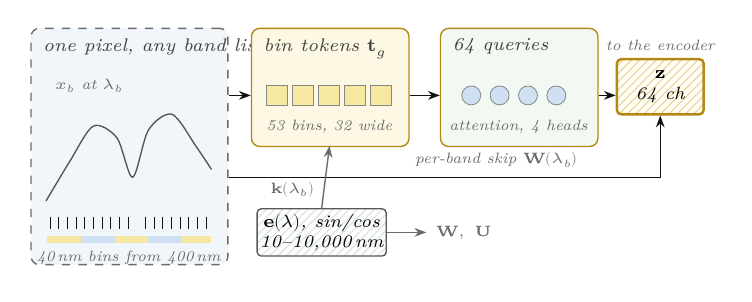
\begin{tikzpicture}[x=1mm,y=1mm]
% spectrum with bands
\node[grp, fill=pB!30, minimum width=25mm, minimum height=30mm, anchor=north west] (GS) at (0,0) {};
\node[glab] at (GS.north west) {one pixel, any band list};
\draw[ink!70, line width=0.5pt] plot[smooth] coordinates {(2,-22) (5,-17) (8,-12.5) (11,-14) (13,-19) (15,-13) (18,-11) (21,-15) (23,-18)};
\foreach \x in {2.5,3.6,4.7,5.8,6.9,8.0,9.1,10.2,11.3,12.4,14.6,15.7,16.8,17.9,19.0,20.1,21.2,22.3} \draw[ink, line width=0.25pt] (\x,-24) -- (\x,-25.6);
\foreach \a/\b/\c in {2.1/6.4/pY,6.4/10.7/pB,10.7/15.0/pY,15.0/19.3/pB,19.3/23.0/pY} \fill[\c] (\a,-26.4) rectangle (\b,-27.4);
\node[tsh] at (12.5,-29.2) {40\,nm bins from 400\,nm};
\node[tsh, anchor=west] at (2,-7.4) {$x_b$ at $\lambda_b$};
% wavelength encoding
\node[stg, pattern color=pB!90, minimum width=15mm, minimum height=6mm] (E) at (37,-26) {$\mathbf e(\lambda)$, sin/cos\\10--10,000\,nm};
% bin tokens
\node[grp, fill=pY!30, draw=ochre!85!black, solid, minimum width=20mm, minimum height=15mm, anchor=north west] (GT) at (28,0) {};
\node[glab] at (GT.north west) {bin tokens $\mathbf t_g$};
\foreach \k in {0,...,4} \node[cell, fill=pY, minimum size=2.6mm] at (31.3+\k*3.3,-8.6) {};
\node[tsh] at (38,-12.6) {53 bins, 32 wide};
% attention
\node[grp, fill=pG!30, draw=ochre!85!black, solid, minimum width=20mm, minimum height=15mm, anchor=north west] (GA) at (52,0) {};
\node[glab] at (GA.north west) {64 queries};
\foreach \k in {0,...,3} \node[cell, circle, fill=pB, minimum size=2.4mm] at (56+\k*3.6,-8.6) {};
\node[tsh] at (62,-12.6) {attention, 4 heads};
% output
\node[stgn, minimum width=11mm, minimum height=7mm] (Z) at (80,-7.5) {$\mathbf z$\\64 ch};
\node[tsh] at (80,-2.2) {to the encoder};
% flows
\draw[df] (GS.east |- 0,-8.6) -- (GT.west |- 0,-8.6);
\draw[df] (GT.east |- 0,-8.6) -- (GA.west |- 0,-8.6);
\draw[df] (GA.east |- 0,-8.6) -- (Z.west |- 0,-8.6);
\draw[df] (GS.east |- 0,-19) -- node[tsh, above, pos=0.62]{per-band skip $\mathbf W(\lambda_b)$} (Z.south |- 0,-19) -- (Z.south);
\draw[df, draw=mute] (E.north) -- node[tsh, left, pos=0.3]{$\mathbf k(\lambda_b)$} (38,-15);
\draw[df, draw=mute] (E.east) -- ++(5,0) node[tsh, right]{$\mathbf W,\ \mathbf U$};
\end{tikzpicture}}

\vspace{0.6mm}
\begin{itemize}\setlength{\itemsep}{0.1mm}\fontsize{6.3}{7.4}\selectfont
\item \textbf{Band-list augmentation}: 80\,\% of batches see a random subset ($\ge$40 bands), wavelengths shifted up to 3\,nm. Before it, native PRISMA: ROC-AUC 0.205, resampled 0.725.
\item 17,825 parameters; $\approx$6$\times$ faster than attention over every band.
\end{itemize}
%% src: R p.3 (80 %, 0.205 vs 0.725), R p.4 (3 nm); docs/lld/spectral-stem.md (min 40 bands; ~6x); 41-heavy.tex (17,825)
\column{0.50\textwidth}
\kicker{the mechanism, per pixel}\par\vspace{-1.6mm}
{\fontsize{7}{8.6}\selectfont\begin{align*}
\mathbf e(\lambda)&=\big[\sin\tfrac{2\pi\lambda}{P_i},\ \cos\tfrac{2\pi\lambda}{P_i}\big]_{i=1}^{16},\qquad P_i\ \text{from 10 to }10^4\,\mathrm{nm}\\
\mathbf t_g&=\big\langle x_b\,\mathbf k(\mathbf e(\lambda_b))\big\rangle_{b\in g}+\boldsymbol\beta\big(\mathbf e(\bar\lambda_g)\big),\qquad g=1,\dots,53\ (40\,\mathrm{nm})\\
z_j&=\mathrm{Attn}\big(\mathbf q_j;\,\{\mathbf t_g\}\big)+\big\langle x_b\,W_j(\mathbf e(\lambda_b))\big\rangle_{\text{all }b},\qquad j=1,\dots,64\\
\hat x(\lambda)&=\mathbf U(\mathbf e(\lambda))\cdot\hat{\mathbf z}+c(\mathbf e(\lambda))\qquad\text{at any requested }\lambda\\
\langle f\rangle_B&=\textstyle\sum_{b\in B}w_bf_b\,\big/\sum_{b\in B}w_b,\qquad w_b=\text{nm band }b\text{ covers}
\end{align*}\par}
\vspace{-1.8mm}
\tx{$x_b$: band $b$'s reflectance, normalised by one fixed curve over wavelength (not per scene). $\mathbf k,\mathbf W,\mathbf U,c$: small networks of $\mathbf e$, so no weight is tied to a band position. 64 learned queries attend over the occupied bins with 4 heads. A token \emph{is} a wavelength range: a band at 1,655\,nm reuses what was learned at 1,650\,nm.}
%% src: app/foundation_models/components/spectral_reduced.py (bin token, width weighting, bin bias, queries, skip, decoder); spectral_tokens.py (periods 10-10,000 nm); F002 config (compressed_channels 64, token_dim 32, heads 4, bin_nm 40, band_weighting width)
\end{columns}
\end{frame}

%======================================================================
% 6 TRAINING
%======================================================================
\begin{frame}{Training}
\begin{columns}[T,onlytextwidth]
\column{0.58\textwidth}
\kicker{two stages on one rented H100 (80\,GB)}\par\vspace{0.3mm}
\fitw{\fontsize{6.4}{7.6}\selectfont\begin{tabular}{@{}l>{\raggedright}p{36mm}>{\raggedright}p{16mm}l>{\raggedright\arraybackslash}p{22mm}@{}}
\toprule
stage & data & model & epochs & settings, time\\
\midrule
pretraining & SpectralEarth (EnMAP), 202 bands; 512,849 training patches, 30,000 per epoch & 33.9\,M & 80 & lr $3\!\times\!10^{-4}$, batch 32, bf16; $\approx$9\,h\\
fine-tuning & EnMAP 210 scenes (14,542 tiles), PRISMA 223 (14,802), AVIRIS-NG 79 lines (22,377); mix 40/35/25\,\% & 35.3\,M (+1.43\,M head) & 10+8+6 & lr $10^{-4}\!\to\!3\!\times\!10^{-5}$; $\approx$5.5\,h\\
selection & four labelled PRISMA scenes & 35.3\,M & ep.\,5 of 6 & epochs 4 / 6: 0.184 / 0.187\\
\bottomrule
\end{tabular}}\par
%% src: R p.4-5 Section 2.2 and Table 4
\vspace{1.4mm}
\kicker{objective, on hidden pixels $M$ (65\,\% of each patch)}\par\vspace{-1.4mm}
\eqs{\[\mathcal L=\underbrace{\tfrac{1}{C|M|}\!\sum_{p\in M}\sum_{c}|\hat x_{c,p}-x_{c,p}|}_{L_1}
+\lambda(t)\,\underbrace{\tfrac{1}{|M|}\!\sum_{p\in M}\angle(\mathbf x_p,\hat{\mathbf x}_p)}_{\text{spectral angle}}
+\,0.1\,\mathcal L_{\mathrm{seg}}\]}
\vspace{-1.6mm}
\tx{$\lambda(t)$ rises 0 $\to$ 0.5 over the first ten epochs; $\mathcal L_{\mathrm{seg}}$ = BCE + Dice, fine-tuning only, shadow and snow $\times$3.}
%% src: R p.4 (loss, ramp), R p.5 (0.1 x BCE + Dice, x3)
\vspace{1.2mm}
\kicker{feeding the GPU}\par\vspace{0.2mm}
\tx{150-patch archives ($\approx$1\,GB, 3,419 for training) read straight from storage gave 18 patches/s; 200 at a time are copied to local disk and swapped every five epochs: 81 patches/s, 18.4\,GB peak, 3,200 archives used. Scenes within 30\,km of the bench are kept out.}
%% src: R p.4-5
\column{0.39\textwidth}
\kicker{pretraining, validation}\par\vspace{0.3mm}
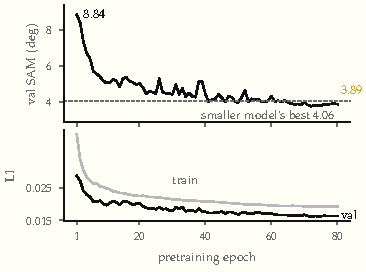
\includegraphics[width=\linewidth]{figures/chart_f002.pdf}\par
%% src: F002-heavy/metrics.csv (plotted); R p.4 (8.84 -> 3.89, 4.06)
\take{Validation spectral angle 8.84$^\circ$ $\to$ 3.89$^\circ$, below the smaller model's best 4.06$^\circ$; epoch 72 seeds fine-tuning.}
\vspace{0.6mm}
\src{Epoch 5 was picked on the bench, so its bench score is slightly optimistic; its neighbours sit within 0.005.}
%% src: R p.5
\end{columns}
\end{frame}

%======================================================================
% 7 DETECTION RESULTS
%======================================================================
\begin{frame}{Detection results}
\kicker{909 labelled objects, four PRISMA scenes, thick cloud excluded; water stays in (vessels are targets)}\par\vspace{0.2mm}
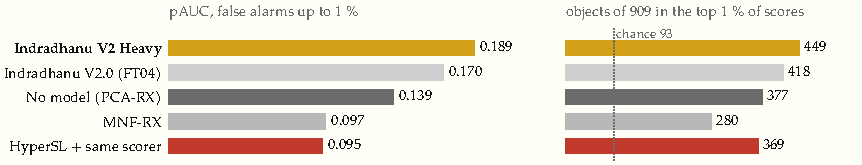
\includegraphics[width=\textwidth]{figures/chart_detection.pdf}\par
%% src: R p.6 Figure 4, Table 5
\vspace{0.6mm}
\begin{columns}[T,onlytextwidth]
\column{0.40\textwidth}
\kicker{the score: residual Mahalanobis}\par\vspace{-1.6mm}
\eqs{\begin{align*}
\mathbf r_p&=\mathbf x_p-\hat{\mathbf x}_p,\qquad \mathbf z_p=\boldsymbol\Lambda_{d}^{-1/2}\mathbf U_{d}^{\top}(\mathbf r_p-\boldsymbol\mu_r),\ d=30\\
s(p)&=\Big\|\mathbf z_p-\tfrac{1}{|\mathcal R_p|}\textstyle\sum_{q\in\mathcal R_p}\mathbf z_q\Big\|^2
\end{align*}}
\vspace{-1.8mm}
\tx{Whiten the residual in its 30 strongest directions; compare with a ring between 21$\times$21 and 61$\times$61. Direction, not size: mean ROC-AUC \textbf{0.662 $\to$ 0.854}, same model.}
%% src: R p.3 (30 directions, 21/61 ring, 0.662 -> 0.854, 3-4 s); research/textbook/chapters/29-residualmaha.tex (equations)
\column{0.29\textwidth}
\kicker{paired bootstrap against FT04}\par\vspace{0.2mm}
\fitw{\fontsize{6.4}{7.6}\selectfont\begin{tabular}{@{}ll@{}}
\toprule
epoch 5 & \textbf{+0.0196} [+0.0072, +0.0316]\\
epoch 4 & +0.0148 [+0.0029, +0.0259]\\
epoch 6 & +0.0179 [+0.0055, +0.0292]\\
no model $-$ V2 & $-$0.047 [$-$0.060, $-$0.033]\\
\bottomrule
\end{tabular}}\par
\vspace{0.6mm}
\tx{Top 1\,\% by tier: easy 58.2 $\to$ \textbf{62.2}, medium 39.3 $\to$ \textbf{43.9}, subtle 40.3 $\to$ \textbf{42.0}\,\%. At top 0.1\,\% the two tie (+0.1 pts).}
%% src: R p.7 (three checks)
\column{0.27\textwidth}
\kicker{per scene, V2 Heavy}\par\vspace{0.2mm}
\fitw{\fontsize{6.4}{7.6}\selectfont\begin{tabular}{@{}lrr@{}}
\toprule
& pAUC & ROC-AUC\\
\midrule
Set-1 & 0.2617 & 0.936\\
Set-2 & 0.1874 & 0.874\\
Set-3 & 0.0861 & 0.781\\
Set-4 & 0.2217 & 0.888\\
\bottomrule
\end{tabular}}\par
\vspace{0.6mm}
\tx{The delivered chain reproduces all four to four decimals. Leaving out thick cloud only: 0.175 $\to$ 0.189.}
%% src: R p.7 (per scene; haze 75.4 %, 209 of 230; 0.175 -> 0.189)
\vspace{0.4mm}
\src{Public benchmark HAD100: appendix A6.}
\end{columns}
\end{frame}

%======================================================================
% 8 DETECTION EXAMPLES
%======================================================================
\begin{frame}{Detection examples}
\begin{columns}[T,onlytextwidth]
\column{0.62\textwidth}
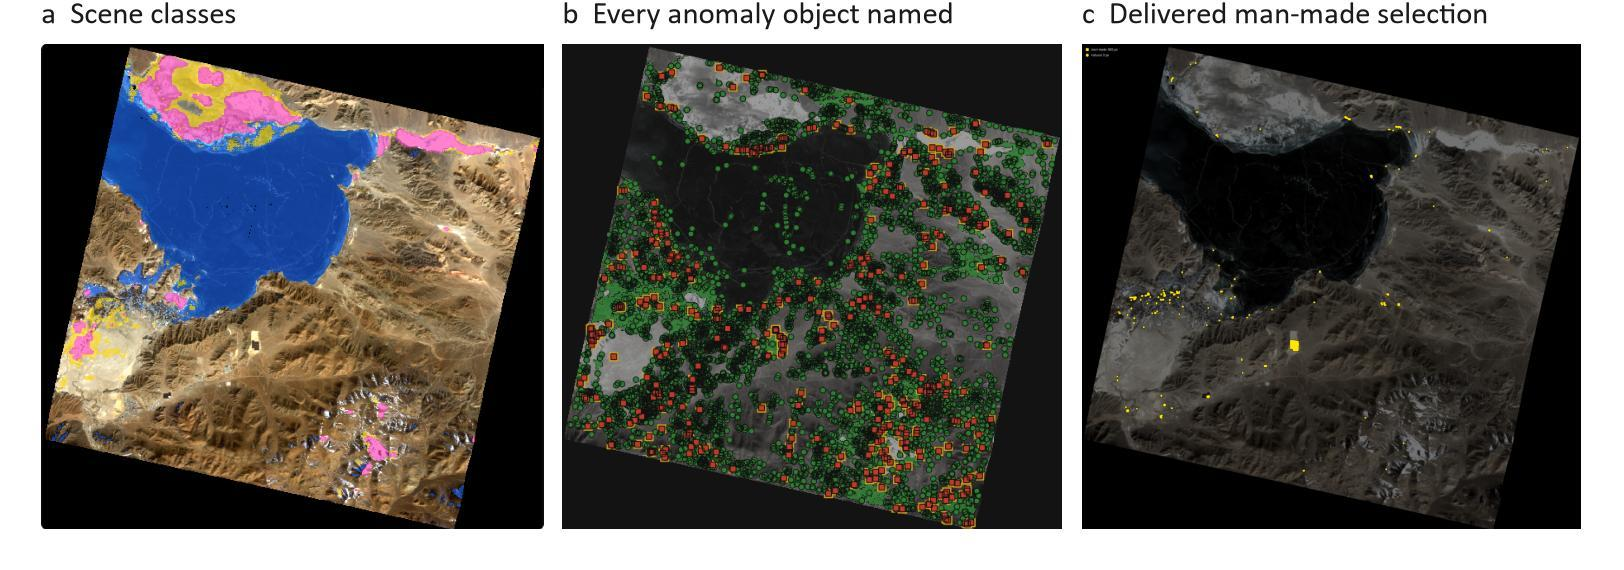
\includegraphics[width=0.82\linewidth]{figures/rep_fig6_prisma.jpg}\par
\src{PRISMA. (a) V2 classes: water blue, cloud pink (left out), haze yellow. (b) 5,544 objects, \mm{} red, \nat{} green. (c) A delivered selection.}
%% src: R p.11 Figure 6
\column{0.35\textwidth}
\kicker{the 405 \mm{} objects}\par\vspace{0.2mm}
\fitw{\fontsize{6.4}{7.6}\selectfont\begin{tabular}{@{}lr@{\hspace{5mm}}lr@{}}
\toprule
concrete/asphalt & 244 & metal & 16\\
oil/fuel & 116 & textile & 3\\
plastic & 25 & wood/paper & 1\\
\bottomrule
\end{tabular}}\par
%% src: R p.11
\vspace{1mm}
\kicker{segmentation head, validation IoU}\par\vspace{0.2mm}
\tx{water 0.825, cloud 0.749. Its thin-cloud class also fires on haze (75.4\,\% of Set-4, 209 of 230 targets), so only thick cloud is left out.}
%% src: R p.3, R p.7
\end{columns}
\vspace{4mm}
\begin{columns}[T,onlytextwidth]
\column{0.40\textwidth}
\kicker{the same chain on three sensors}\par\vspace{0.2mm}
\fitw{\fontsize{6.4}{7.6}\selectfont\begin{tabular}{@{}lrrr@{}}
\toprule
& Tanager & PRISMA & AVIRIS-NG\\
\midrule
anomaly objects & 1,103 & 5,544 & 2,375\\
\mm{}, $P>0.5$ & 272 & 405 & 1,290\\
\mm{}, $P>0.25$ & 585 & 2,263 & 1,716\\
oil/fuel or plastic & 247 & 141 & 936\\
\bottomrule
\end{tabular}}\par
%% src: R p.11 Table 8
\vspace{0.6mm}
\tx{Tanager was never in training; GHOSt (Golmud, 8\,m) ran end to end on evaluation day.}
\column{0.58\textwidth}
\setlength{\tabcolsep}{0.5mm}
\begin{tabular}{@{}cccc@{}}
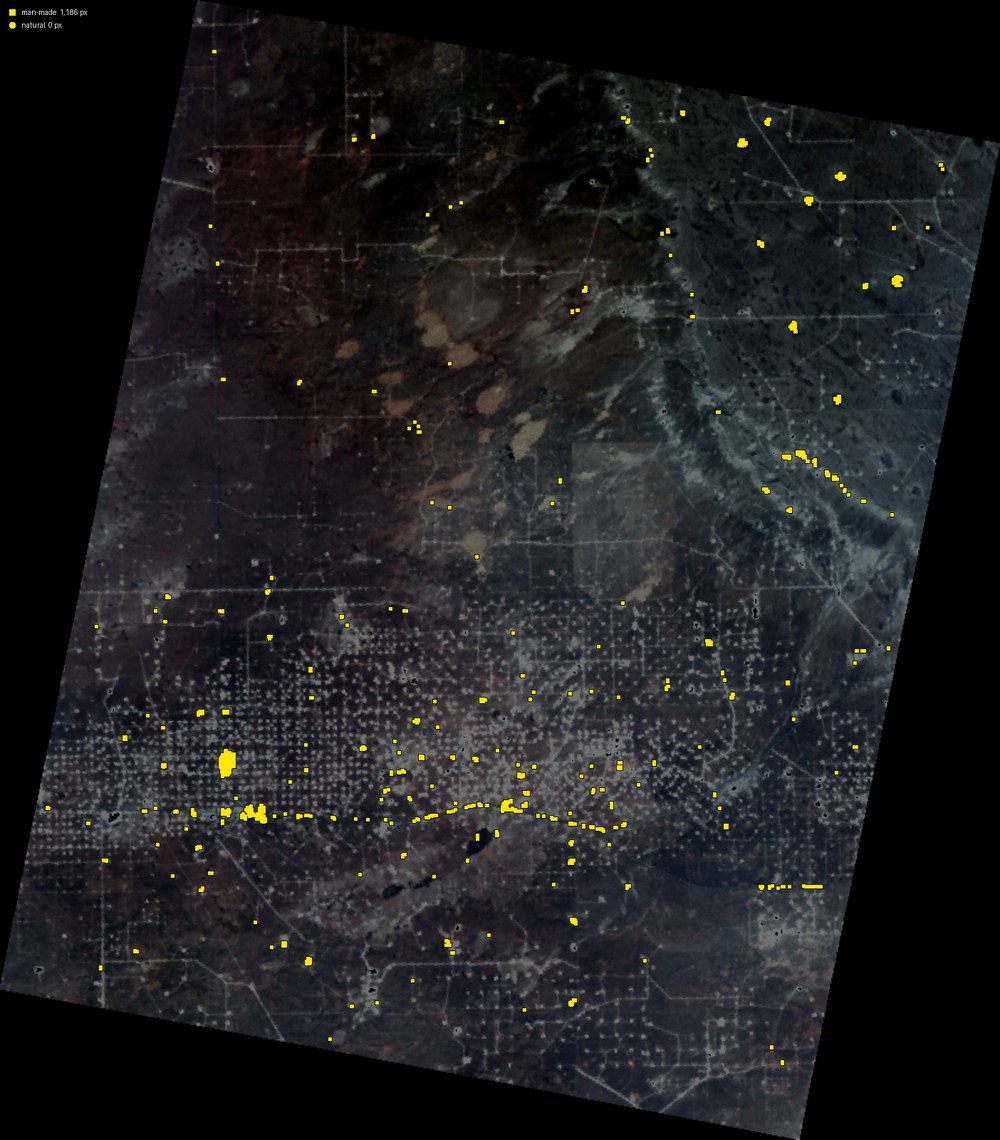
\includegraphics[height=23mm]{figures/ql_tanager_manmade.jpg}&
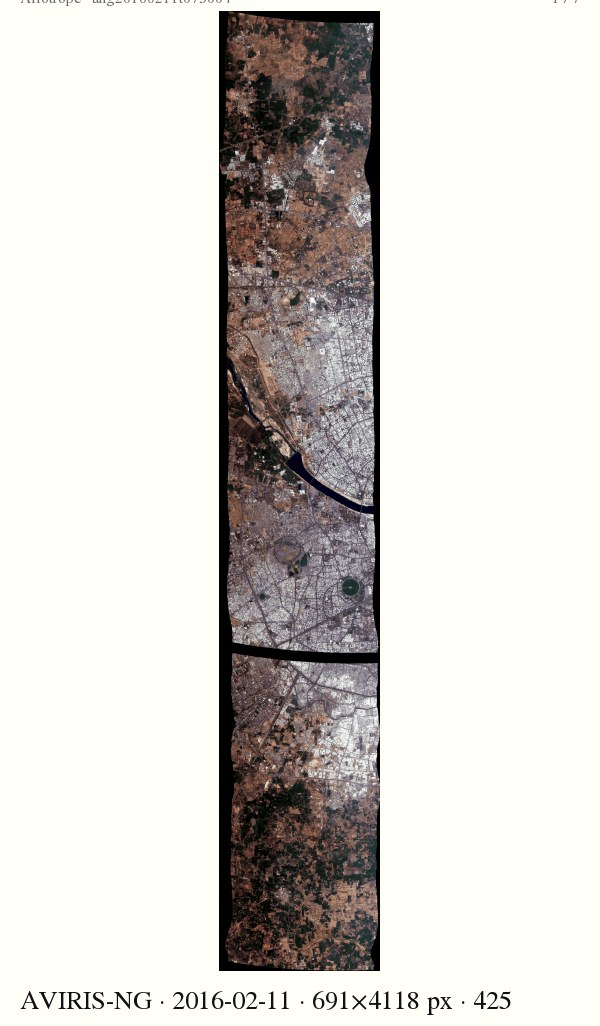
\includegraphics[height=23mm]{figures/story_aviris_k1.jpg}&
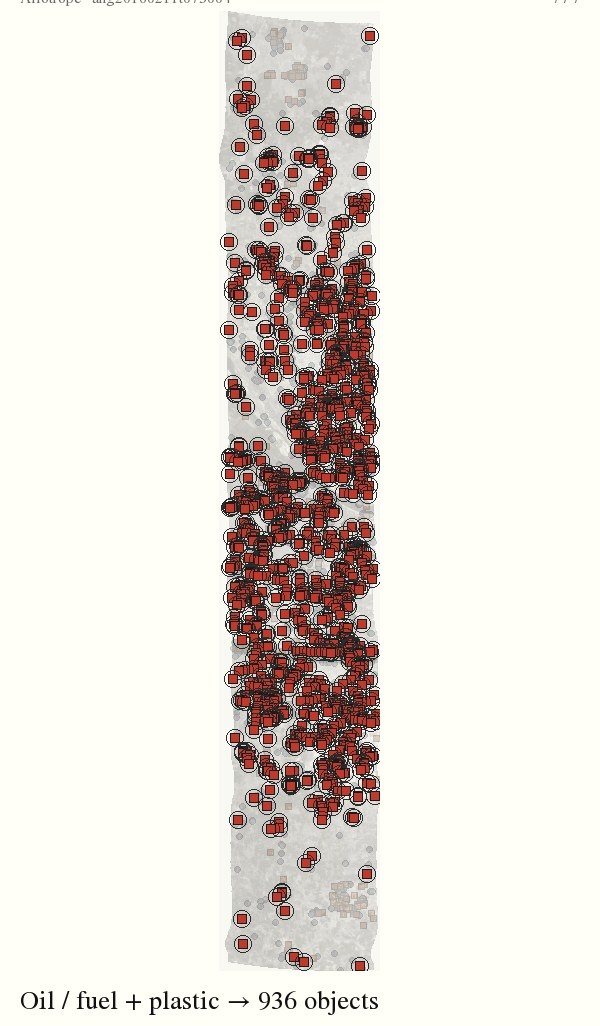
\includegraphics[height=23mm]{figures/story_aviris_k7.jpg}&
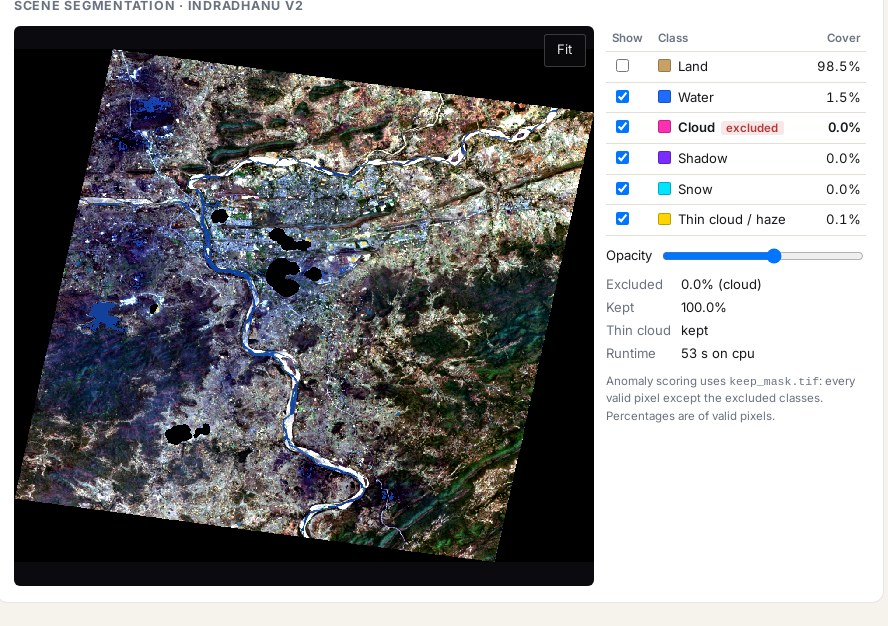
\includegraphics[height=23mm]{figures/seg_enmap_panel.jpg}\\[-0.6mm]
\srcc{Tanager, man-made}&\srcc{AVIRIS-NG}&\srcc{oil + plastic}&\srcc{EnMAP, classes}
\end{tabular}
\end{columns}
\end{frame}

%======================================================================
% 9 ATMOSPHERIC CORRECTION
%======================================================================
\begin{frame}{Atmospheric correction}
\centering
% Atmospheric-correction chain, NAS-figure style. Stages and roles from the report's ATM section
% ("Key modules: radiometric vs atmospheric correction", pp. 17-18); ISOFIT 4.1.5 + sRTMnet from the container README.
\adjustbox{max width=\textwidth}{%
\begin{tikzpicture}[x=1mm,y=1mm]
\tikzset{ab/.style={stg, minimum width=17mm, minimum height=13mm, text width=17mm, font=\fontsize{5.9}{6.8}\selectfont}}
\node[inner sep=0, anchor=west] (in) at (0,-12) {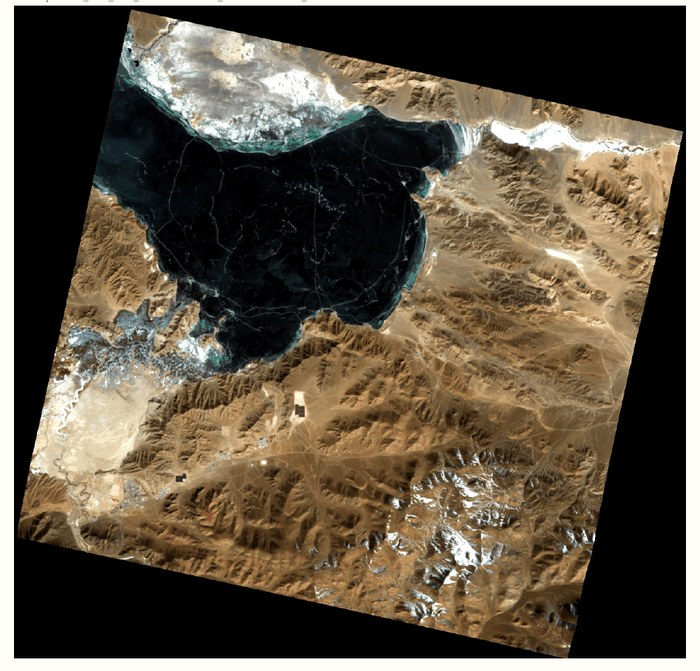
\includegraphics[width=10mm]{figures/story_prisma_k1.jpg}};
\node[tsh, below=0.2mm of in, align=center] {L1 radiance\\or TOA, any file};
% radiometric
\node[grp, fill=pB!35, minimum width=40mm, minimum height=19mm, anchor=north west] (G1) at (14,-1) {};
\node[glab] at (G1.north west) {Radiometric};
\node[ab, pattern color=pB!90] (r1) at (24,-12.5) {\textbf{\upshape Read}\\\upshape native or generic; level detected, not assumed};
\node[ab, pattern color=pB!90] (r2) at (44,-12.5) {\textbf{\upshape To radiance}\\\upshape gain, offset, scale per sensor};
% atmospheric
\node[grp, fill=pG!35, minimum width=61mm, minimum height=19mm, anchor=north west] (G2) at (57,-1) {};
\node[glab] at (G2.north west) {Atmospheric (ISOFIT 4.1.5)};
\node[ab, pattern color=pG!90] (a1) at (67,-12.5) {\textbf{\upshape Look-up table}\\\upshape 6S + sRTMnet; AOT, H$_2$O, elevation, geometry};
\node[ab, pattern color=pG!90] (a2) at (87.5,-12.5) {\textbf{\upshape Optimal}\\\textbf{\upshape estimation}\\\upshape on superpixels; surface prior};
\node[ab, pattern color=pG!90] (a3) at (108,-12.5) {\textbf{\upshape Every pixel}\\\upshape analytical or empirical line, GPU};
% surface
\node[grp, fill=pY!35, minimum width=40mm, minimum height=19mm, anchor=north west] (G3) at (121,-1) {};
\node[glab] at (G3.north west) {Surface};
\node[ab, pattern color=pY!95] (s1) at (131,-12.5) {\textbf{\upshape Post}\\\upshape outliers, terrain, adjacency, snow};
\node[stgn, minimum width=17mm, minimum height=11mm, text width=17mm, font=\fontsize{5.9}{6.8}\selectfont, pattern color=pY!95] (s2) at (151,-12.5) {\textbf{\upshape Harmonise}\\\upshape towards the vendor L2, per sensor};
% output
\node[stg, pattern color=pR!90, minimum width=17mm, minimum height=11mm, text width=17mm, font=\fontsize{5.9}{6.8}\selectfont] (o) at (174,-12.5) {\textbf{\upshape L2 surface reflectance}\\\upshape GeoTIFF + BSQ, wavelengths};
% DEM
\node[stg, pattern color=faint!50, minimum width=14mm, minimum height=5mm, font=\fontsize{5.6}{6.6}\selectfont] (dem) at (87.5,-27) {\upshape Copernicus DEM};
\node[loss] (ref) at (151,-27) {vendor L2 (fit only)};
\draw[df] (in) -- (r1); \draw[df] (r1) -- (r2); \draw[df] (r2) -- (a1); \draw[df] (a1) -- (a2); \draw[df] (a2) -- (a3);
\draw[df] (a3) -- (s1); \draw[df] (s1) -- (s2); \draw[df] (s2) -- (o);
\draw[df] (dem.west) -| (a1.south); \draw[df] (dem.east) -| (s1.south);
\draw[tf] (ref) -- (s2);
\end{tikzpicture}}

%% src: R p.17-18 (modules, radiometric vs atmospheric); container README (ISOFIT 4.1.5 + sRTMnet)
\vspace{0.4mm}
\begin{columns}[T,onlytextwidth]
\column{0.50\textwidth}
\kicker{radiance model and optimal estimation}\par\vspace{-1.6mm}
{\fontsize{7.2}{8.8}\selectfont\begin{align*}
\rho_{\mathrm{TOA}}&=\frac{\pi d^2 L}{E_0\cos\theta_s}=\rho_{\mathrm{path}}+\frac{T^{\downarrow}T^{\uparrow}\rho_s}{1-S\rho_s}\\
\hat{\mathbf x}&=\arg\min_{\mathbf x}\ \big\|\mathbf y-F(\mathbf x)\big\|^2_{\mathbf S_\epsilon^{-1}}+\big\|\mathbf x-\mathbf x_a\big\|^2_{\mathbf S_a^{-1}}
\end{align*}\par}
\vspace{-1.8mm}
\tx{State $\mathbf x$: surface reflectance $\rho_s(\lambda)$, aerosol optical thickness, water vapour. $F$: the look-up-table forward model; $\mathbf x_a,\mathbf S_a$: surface prior; $\mathbf S_\epsilon$: instrument noise. Adjacency: $\rho=\rho_{\mathrm{ret}}+q(\rho_{\mathrm{ret}}-\rho_{\mathrm{bg}})$, 1\,km kernel.}
%% src: R p.17-18 (TOA conversion rho E0 cos / (pi d^2); adjacency formula); ISOFIT optimal-estimation formulation (Thompson et al. 2018)
\vspace{0.6mm}
\tx{Inverts within 350--1360, 1410--1800, 1970--2500\,nm. Superpixels of 50 for satellites; 400 with an empirical line for 4--16\,Mpix AVIRIS-NG lines.}
%% src: R p.18 Band handling
\column{0.46\textwidth}
\kicker{per-sensor rules}\par\vspace{0.2mm}
\fitw{\fontsize{6.2}{7.4}\selectfont\begin{tabular}{@{}l>{\raggedright}p{19mm}>{\raggedright}p{15mm}>{\raggedright}p{11mm}r@{}}
\toprule
sensor & to radiance & aerosol & terrain, adjacency & bands kept\\
\midrule
PRISMA & DN / scale $-$ offset; VNIR/SWIR split 950\,nm & NASA POWER climatology $\pm$0.15 & off & 206\\
EnMAP & DN $\times$ gain + offset & free, seasonal limits & on & 218\\
AVIRIS-NG & units only & 0.10--0.14, as JPL & off & 380\\
Tanager & units only & free, seasonal limits & on & 382\\
\bottomrule
\end{tabular}}\par
%% src: R p.18 (radiometric bullets, AOT bullets, bands kept); R p.18-19 terrain/adjacency table (terrain EnMAP, Tanager only when >1 % steeper than 6 deg; adjacency EnMAP, Tanager below 2 km; off for PRISMA, AVIRIS-NG, GHOSt)
\vspace{0.6mm}
\tx{Terrain only where the vendor does it: SWIR $r$ 0.947 $\to$ 0.980 on mountains. Snow by NDSI (precision 0.91--1.00). Reflectance $>2.5$ kept and flagged: flares and fires are anomalies.}
%% src: R p.18-19
\end{columns}
\end{frame}

%======================================================================
% 10 CORRECTION ACCURACY
%======================================================================
\begin{frame}{Correction accuracy}
\begin{columns}[T,onlytextwidth]
\column{0.47\textwidth}
\kicker{held-out scenes against the vendor L2, 460--2450\,nm core}\par\vspace{0.3mm}
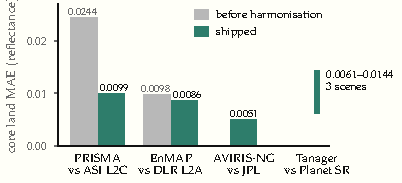
\includegraphics[width=\linewidth]{figures/chart_atm_mae.pdf}\par
%% src: R p.19 Harmonisation table
\vspace{0.4mm}
\tx{Two good L2 products differ by 0.01--0.02. A per-sensor model of the retrieved atmosphere (AOT, H$_2$O, sun zenith, elevation) maps ours to the vendor's; fitted on 15--27 scenes, scored once on 5 held-out. PRISMA: all five improved. EnMAP: blue bands only, 460\,nm bias +0.023 $\to$ +0.001.}
%% src: R p.19
\src{EnMAP's blue range was chosen after the held-out scores were seen. Aim: one reflectance domain, so one anomaly model serves every sensor.}
\column{0.50\textwidth}
\kicker{run time per scene}\par\vspace{0.3mm}
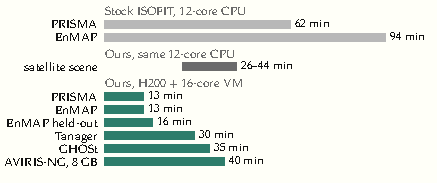
\includegraphics[width=\linewidth]{figures/chart_atm_time.pdf}\par
%% src: R p.19-20 Measured run times
\vspace{0.4mm}
\kicker{how}\par\vspace{0.1mm}
\fitw{\fontsize{6.4}{7.6}\selectfont\begin{tabular}{@{}l>{\raggedright\arraybackslash}p{56mm}@{}}
\toprule
exact & 6S aerosol-only call removed (1.9$\times$), scattering cached over water vapour (5$\times$); GPU per-pixel solve 3.2$\times$, difference $\le$6$\times$10$^{-8}$\\
measured & EnMAP prior on true band centres 53 $\to$ 30 min; AVIRIS-NG superpixels 400: window 40.8 $\to$ 7.5 min, error 0.0056 $\to$ 0.0057; full 4\,Mpix line 373 $\to$ 41 min\\
robust & input level detected by O$_2$/H$_2$O absorption tests, 28/28 right; ambiguity stops the run and names the fix\\
\bottomrule
\end{tabular}}\par
%% src: R p.18 (superpixels), R p.19 (speed-ups), R p.20 (robustness)
\end{columns}
\end{frame}

%======================================================================
% 11 MATERIAL IDENTIFICATION
%======================================================================
\begin{frame}{Material identification}
\begin{columns}[T,onlytextwidth]
\column{0.37\textwidth}
\kicker{two matchers on every detected pixel}\par\vspace{0.2mm}
\tx{USGS splib07 + ECOSTRESS, resampled to the sensor: seven \mm{} classes (oil/fuel, plastic, textile, wood/paper, paint, metal, concrete/asphalt) and a \nat{} shelf; 378 / 338 / 380 spectra (EnMAP / PRISMA / AVIRIS-NG).}
%% src: R p.9
\vspace{0.8mm}
\tx{\textbf{SAM}: smallest angle $\theta_j=\arccos\frac{\mathbf x\cdot\mathbf s_j}{\|\mathbf x\|\|\mathbf s_j\|}$; no training, but blind to the ground filling the rest of the pixel.}
\vspace{0.6mm}
\tx{\textbf{Spectral namer} (347,685 parameters) on \textbf{V2's spectral stem}: one tower reads the pixel and its ring mean (3--7\,px away), the other the library.}
\vspace{-1.6mm}
\eqs{\begin{align*}
s_j&=\cos(\mathbf z,\mathbf e_j)/\tau,\quad S_c=\log\textstyle\sum_{j\in c}e^{s_j}\\
P(\text{\mm})&=\sigma\big(\operatorname{LSE}_{c\ne\text{nat}}S_c-S_{\text{nat}}+b\big)
\end{align*}}
\vspace{-2mm}
\tx{Level 1: share of the match on \mm{} spectra; level 2: best class. Trained on library spectra planted at 5--100\,\% fill in real EnMAP, PRISMA, AVIRIS-NG pixels, 20\,\% of each class held out. New spectra need no retraining.}
%% src: R p.9 4.1; research/textbook/chapters/42-namer.tex (s_j, S_c; level 1 = share identity)
\column{0.33\textwidth}
\kicker{level 1 at ACE's false-alarm rate}\par\vspace{0.2mm}
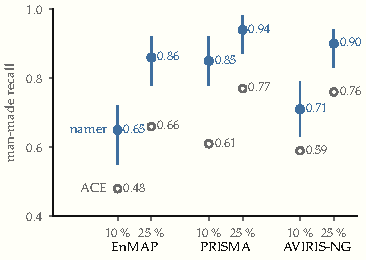
\includegraphics[width=\linewidth]{figures/chart_namer_ace.pdf}\par
%% src: R p.10 Figure 5
\take{Quarter-pixel fill: 86--94\,\% of \mm{} targets found; ACE 66--77\,\%.}
\column{0.26\textwidth}
\kicker{level 2, class correct}\par\vspace{0.2mm}
\fitw{\fontsize{6.4}{7.6}\selectfont\begin{tabular}{@{}lll@{}}
\toprule
fill 10\,\% & namer & ACE\\
\midrule
EnMAP & \textbf{0.59} [0.48, 0.70] & 0.24\\
PRISMA & \textbf{0.69} [0.53, 0.81] & 0.41\\
AVIRIS-NG & \textbf{0.65} [0.53, 0.76] & 0.38\\
\midrule
fill 25\,\% & & \\
EnMAP & \textbf{0.68} [0.55, 0.79] & 0.47\\
PRISMA & 0.70 [0.54, 0.82] & 0.60\\
AVIRIS-NG & 0.70 [0.57, 0.82] & 0.58\\
\bottomrule
\end{tabular}}\par
%% src: R p.10 Table 6
\vspace{0.6mm}
\tx{Planted sub-pixel targets in PRISMA scenes, 10\,\% fill, 8 classes: namer \textbf{0.53}; best training-free 0.44; HyperSL-based 0.27--0.30.}
%% src: R p.1, R p.14 Table 12
\end{columns}
\end{frame}

%======================================================================
% 12 FIELD TARGETS
%======================================================================
\begin{frame}{Field targets}
\begin{columns}[T,onlytextwidth]
\column{0.34\textwidth}
\kicker{real targets laid out in the field}\par\vspace{0.3mm}
\tx{\textbf{HySU} (DLR, airborne, 0.7\,m): bitumen, red-painted metal, blue, red and green synthetic fabric, squares 0.25--3\,m; 135 bands, 417--903\,nm, a range the namer never trained on. 22 targets, 236 target pixels, 3,000 background.}
\vspace{0.8mm}
\tx{\textbf{Gudalur} (AVIRIS-NG, Nilgiris 2018, 4\,m): five 16$\times$16\,m sheets (green, red, yellow, black nylon; white cotton) with field spectra; 80 pixels, 353 bands. Also coarsened to 32\,m at four offsets: each sheet $\le$ a quarter pixel, 27 pixels (anecdotal).}
\vspace{0.8mm}
\tx{Namer here has textile held out, so textile is unseen; nylon may count as plastic or textile, bitumen as concrete or oil.}
%% src: R p.11-12 Section 4.4
\column{0.63\textwidth}
\kicker{level 2: class correct, shared library and with the site's own spectra}\par\vspace{0.3mm}
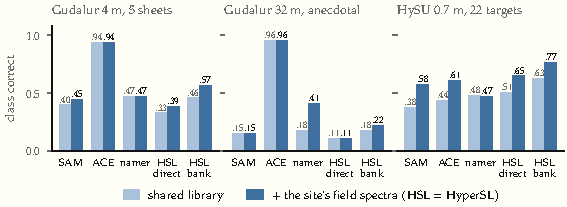
\includegraphics[width=\linewidth]{figures/chart_field.pdf}\par
%% src: R p.12 Table 9 / Figure 7
\vspace{0.6mm}
\fitw{\fontsize{6.4}{7.6}\selectfont\begin{tabular}{@{}lccc@{}}
\toprule
level 1: AUC of the \mm{} call & Gudalur 4\,m & Gudalur 32\,m & HySU\\
\midrule
SAM & 0.69 / 0.70 & 0.39 / 0.39 & 0.65 / 0.73\\
ACE & 0.58 / \textbf{0.89} & 0.58 / \textbf{0.86} & 0.63 / \textbf{0.81}\\
spectral namer & 0.15 / 0.15 & 0.17 / 0.18 & 0.58 / 0.61\\
HyperSL, mixture bank & 0.51 / 0.59 & 0.15 / 0.19 & 0.57 / 0.80\\
\bottomrule
\end{tabular}}\par
%% src: R p.12 Table 9
\vspace{0.6mm}
\tx{ACE names the Gudalur sheets best (5 of 5 at 4\,m, 18 of 19 at 32\,m). The namer's \mm{} call is \emph{inverted} on the sheets: a 16\,m sheet is not a pixel unlike its ring. On HySU the HyperSL mixture bank names the most (16 of 22; 18 with field spectra). Small sets: examples, not rates.}
%% src: R p.12
\end{columns}
\end{frame}

%======================================================================
% 13 AGAINST HYPERSL
%======================================================================
\begin{frame}{Against HyperSL}
\begin{columns}[T,onlytextwidth]
\column{0.44\textwidth}
\kicker{a public spectral foundation model, run unmodified}\par\vspace{0.2mm}
\tx{Per-pixel masked autoencoder, 9.2\,M parameters, EnMAP and DESIS reflectance; hides 95\,\% of a pixel's bands and rebuilds them from the same pixel.}
\vspace{0.8mm}
\tx{\textbf{1 Self-reconstruction.} An unusual pixel rebuilds as well as an ordinary one: its own loss as a score finds 63 objects, fewer than random (93). Indradhanu hides whole pixels.}
\vspace{0.4mm}
\tx{\textbf{2 Per-scene min-max.} $x'_b=(x_b-m_b)/(M_b-m_b)$ from the scene: (0.20, 0.50) becomes (0.5, 1.0) in one scene, (0.43, 0.75) in another; an angle moves 15.1$^\circ$ $\to$ 36.9$^\circ$ with no change in reflectance. A library spectrum has no scene: 41\,\% of ECOSTRESS values clipped.}
\vspace{0.4mm}
\tx{\textbf{3 Band order, not wavelength.} List neighbours straddle water-vapour gaps and differ per sensor. Indradhanu bins by wavelength.}
\vspace{0.4mm}
\tx{\textbf{4 Cloud-free pretraining.} Cirrus recall 28.9\,\% from its features against 67.9\,\% from raw bands.}
%% src: R p.12-13 Section 5.1
\column{0.53\textwidth}
\kicker{same bench, same scorer, all pixels}\par\vspace{0.2mm}
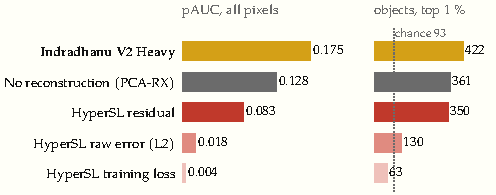
\includegraphics[width=\linewidth]{figures/chart_hypersl.pdf}\par
%% src: R p.13 Figure 8
\vspace{0.2mm}
\fitw{\fontsize{6.4}{7.6}\selectfont\begin{tabular}{@{}lll@{}}
\toprule
paired difference [95\,\%] & pAUC & objects (pts)\\
\midrule
HyperSL $-$ no model & $-$0.045 [$-$0.059, $-$0.032] & $-$1.2 [$-$4.0, +1.5]\\
HyperSL $-$ V2 Heavy & $-$0.092 [$-$0.106, $-$0.078] & $-$7.9 [$-$10.8, $-$5.2]\\
\bottomrule
\end{tabular}}\par
%% src: R p.13 Table 10
\vspace{0.8mm}
\fitw{\fontsize{6.4}{7.6}\selectfont\begin{tabular}{@{}lcccc@{}}
\toprule
unmixing RMSE, true endmembers & DC1 / DC2 / DC3 & EGU & Jasper & Urban\\
\midrule
reflectance, best physical & 0.000 / 0.000 / 0.000 & 0.018 & 0.050 & 0.059\\
HyperSL internal space & 0.253 / 0.113 / 0.261 & 0.142 & 0.106 & 0.170\\
\bottomrule
\end{tabular}}\par
%% src: R p.13 Table 11
\take{Not adopted: it lowers detection below no model, bends mixing (0.4--0.7 of the path length), and its matching trails plain reflectance.}
%% src: R p.13-14
\end{columns}
\end{frame}

%======================================================================
% 14 DELIVERABLES AND LIMITS
%======================================================================
\begin{frame}{Deliverables and limits}
\begin{columns}[T,onlytextwidth]
\column{0.30\textwidth}
\kicker{per scene and selection}\par\vspace{0.2mm}
\begin{itemize}\setlength{\itemsep}{0.2mm}\fontsize{6.4}{7.6}\selectfont
\item Boolean anomaly mask, GeoTIFF, 0/1 on the scene's own UTM grid; \textbf{no heatmap}.
\item Pixel and object shapefiles and a table, latitude and longitude.
\item Every pixel and object: namer call, class and confidence, ACE family match, best SAM match and its angle.
\item L2 surface reflectance from L1, GeoTIFF and BSQ with wavelengths.
\end{itemize}
%% src: R p.15 (delivered files carry namer call, class, confidence, ACE family, SAM match + angle); docs/lld/spectral-namer-in-product.md (pack)
\vspace{0.8mm}
\kicker{on the evaluation VM}\par\vspace{0.2mm}
\fitw{\fontsize{6.4}{7.6}\selectfont\begin{tabular}{@{}lll@{}}
\toprule
& scoring & L1 $\to$ L2\\
\midrule
time & $<$30\,s & 16 min\\
CPU, 16 cores & $\approx$10\,\% & $\approx$90\,\% peak\\
RAM, 64\,GB & $\approx$24\,\% & $\approx$10\,\%\\
GPU, H200 & $\approx$3\,\% & $\approx$4\,\%\\
\bottomrule
\end{tabular}}\par
%% src: R p.21 Hardware Requirements
\column{0.36\textwidth}
\kicker{evaluation scene: GHOSt, Golmud airport}\par\vspace{0.2mm}
\tx{GeoTIFF input; airstrip, a smaller field and buildings on bare soil; visible striping. Two scorings: Heavy + RX hybrid, and Heavy alone. Natural calls removed: $\approx$8,000 $\to$ $\approx$3,000 and $\approx$5,500 $\to$ $\approx$3,700 pixels submitted.}
\vspace{0.4mm}
\fitw{\fontsize{6.2}{7.4}\selectfont\begin{tabular}{@{}lrrll@{}}
\toprule
\mm{} class & sub.\,1 & sub.\,2 & namer's match & SAM's match\\
\midrule
plastic & 39.6 & 30.3 & fiberglass & cerium oxide\\
metal & 24.2 & 21.8 & coated steel girder & calcite\\
concrete/asphalt & 23.1 & 23.4 & construction concrete & lead white\\
oil/fuel & 7.7 & 16.8 & oiled marsh plant & buckbrush\\
textile & 2.2 & 3.7 & terrycloth fabric & grass\\
wood/paper & 2.2 & 3.7 & particle board & grass\\
paint & 1.1 & 0.3 & olive green paint & grass\\
\bottomrule
\end{tabular}}\par
%% src: R p.20-21 Section 10 (both submission tables; SAM column from submission 1)
\vspace{0.3mm}
\src{Share of \mm{} pixels, \%. SAM's nearest spectra are minerals and plants.}
\column{0.30\textwidth}
\kicker{limits}\par\vspace{0.2mm}
\begin{itemize}\setlength{\itemsep}{0.2mm}\fontsize{6.4}{7.6}\selectfont
\item \textbf{Large targets.} The namer compares a pixel with its ring; roads, roofs and big sheets defeat it. SAM and ACE guide there.
\item \textbf{Open set.} Unseen textile: 46--47\,\% still called \mm{}, then a confident wrong class; abstention flags 1--4\,\%. In-scene solar panels changed nothing (0.248 $\to$ 0.248).
\item \textbf{Small sets.} 5 sheets at Gudalur, 22 targets at HySU; four PRISMA scenes, $\pm$0.005--0.01 pAUC.
\item \textbf{Threshold} is an analyst choice; the evaluation scenes have no ground truth.
\item \textbf{Cost.} Heavy 454\,s per PRISMA scene on CPU, FT04 274\,s.
\end{itemize}
%% src: R p.15 Section 7
\src{Next: field spectra for camouflage and coatings, a glass and solar-panel class, a labelled bench beyond PRISMA.}
%% src: R p.16
\end{columns}
\end{frame}

%======================================================================
% 15 JOURNEY
%======================================================================
\begin{frame}{Journey}
\centering
\resizebox{\textwidth}{!}{%
\begin{tikzpicture}[x=1mm,y=1mm, every node/.append style={execute at begin node={\hyphenpenalty=10000\exhyphenpenalty=10000}}]
% phase bands (x is piecewise: Jan-Aug compressed, October expanded; breaks drawn on the axis)
\fill[band] (-1,-31) rectangle (34,25);
\fill[band!55] (34.6,-31) rectangle (60,25);
\fill[band] (60.6,-31) rectangle (121,25);
\fill[band!55] (121.6,-31) rectangle (149,25);
\foreach \x/\t in {16.5/Foundation, 47.3/Product, 90.8/Detection, 135.3/Material}
  \node[font=\scshape\fontsize{6.6}{7}\selectfont, color=mute] at (\x,22.8) {\t};
% axis
\draw[ink, line width=0.4pt] (-1,0) -- (149,0);
\foreach \x/\d in {0/Jan,10/Mar,20/Apr,30/May,36/Jul,48/Aug,62/14 Oct,80/19 Oct,98/22 Oct,112/29 Oct,128/31 Oct,146/1 Nov}
  {\draw[ink] (\x,0) -- (\x,-0.9); \node[font=\fontsize{5.6}{6}\selectfont, color=mute, below] at (\x,-0.9) {\d};}
\foreach \b in {34.3,60.3} {\fill[band] (\b-0.9,-1.2) rectangle (\b+0.9,1.2);
  \draw[ink] (\b-1.4,-1.2) -- (\b-0.4,1.2); \draw[ink] (\b+0.4,-1.2) -- (\b+1.4,1.2);}
% milestones (above)
\foreach \x/\h/\w/\t in {
 {0/12/17mm/{\textbf{26 Jan} first\\commit: HE5 and\\TIF readers}},
 {10/4/9mm/{\textbf{23 Mar}\\first\\trainer}},
 {20/12/13mm/{\textbf{10 Apr}\\hyperspectral\\SegFormer MAE}},
 {36/4/22mm/{\textbf{23 Jul} backend +\\frontend: the app}},
 {62/12/17mm/{\textbf{14 Oct} Spectral-\\Earth pretraining,\\wavelength stem}},
 {66/3/13mm/{\textbf{15 Oct}\\residual\\Mahalanobis}},
 {80/12/17mm/{\textbf{19 Oct} FT04\\ships as V2,\\pAUC 0.170}},
 {106/12/18mm/{\textbf{28--29 Oct}\\Heavy on an H100:\\0.189, v2.1.0}},
 {128/12/13mm/{\textbf{31 Oct}\\namer N001b\\passes level 1}}}
 {\draw[ink, line width=0.35pt] (\x,0) -- (\x,\h); \fill[ink] (\x,0) circle (0.7); \node[ms=\w] at (\x+0.6,\h-0.6) {\t};}
\draw[ochre, line width=0.6pt] (146,0) -- (146,4); \fill[ochre] (146,0) circle (1.1);
\node[font=\fontsize{7}{8}\selectfont, anchor=south east, align=right] at (148,4.3) {\textbf{v1.0}};
% failures (below): x, level, width, text
\foreach \x/\h/\w/\t in {
 {30/-5/17mm/{\textbf{May} plain RX\\fails: covariance\\near singular,\\distances $10^{11}$\\$\to$ MNF-RX}},
 {48/-5/12.5mm/{\textbf{Aug} two\\outages hit\\main; fake\\docs removed\\$\to$ check\\the worker}},
 {98/-5/13mm/{\textbf{22 Oct} FT07,\\FT08: 0.165,\\0.164 $<$ 0.170\\$\to$ widen\\the model}},
 {112/-5/11mm/{\textbf{29 Oct}\\haze read\\as cloud:\\209 of 230\\targets $\to$\\thick only}},
 {124/-17/13mm/{\textbf{31 Oct}\\HyperSL:\\0.083 $<$ 0.128\\$\to$ rejected}},
 {130/-5/13mm/{\textbf{31 Oct}\\N001 level 1\\at chance\\(0.50) $\to$\\matching}}}
 {\draw[manmade!60, line width=0.35pt] (\x,-3.3) -- (\x,\h); \draw[manmade, line width=0.5pt] (\x-0.7,-0.7) -- (\x+0.7,0.7) (\x-0.7,0.7) -- (\x+0.7,-0.7); \node[fl=\w] at (\x+0.6,\h+0.6) {\t};}
\draw[manmade!60, line width=0.35pt] (146,-3.3) -- (146,-17);
\draw[manmade, line width=0.5pt] (145.3,-0.7) -- (146.7,0.7) (145.3,0.7) -- (146.7,-0.7);
\node[fl=10mm, anchor=north east, align=right] at (147.5,-17.6) {\textbf{1 Nov}\\PV spectra:\\no effect};
% pAUC sparkline (matplotlib, figures/chart_spark.pdf)
\node[anchor=south west, inner sep=0] at (63,-30) {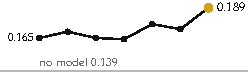
\includegraphics[width=42mm]{figures/chart_spark.pdf}};
\node[font=\fontsize{5.6}{6}\selectfont, color=mute, anchor=north west] at (64,-30.3) {pAUC: v0.2.0, FT04, FT07, FT08, FT09b, FT09c, Heavy};
\end{tikzpicture}}

%% src dates: git log (see NUMBERS.md); failures: CLAUDE.md, docs/lld/evaluation.md, docs/lld/spectral-stem.md, hypersl-anomaly-bench README, N001 README, pv-library README
\vspace{0.3mm}
{\small From a spatial pipeline to a spectral foundation model: \textbf{any sensor in, materials out.}\par}
\end{frame}

%======================================================================
% APPENDIX
%======================================================================
\appendix
\renewcommand{\decklabel}{AIGC Stage III \textperiodcentered{} appendix}

\begin{frame}{A1 Model generations}
\centering
% Architecture evolution of Indradhanu: one mini schematic per generation; new parts in ochre.
% Sources: docs/04-models.md, docs/lld/spectral-stem.md, docs/lld/evaluation.md, research/experiments/indradhanu-se-pretrain/F002-heavy/README.md,
% research/experiments/indradhanu-finetune/FTH3-heavy-joint-more2/README.md, final design/ROADMAP.md (OB-14), git log dates.
\newcommand{\gen}[8]{% x, input, stem style, stem, encoder style, encoder, decoder style, decoder
  \node[lab, color=mute] at (#1,0) {#2};
  \node[#3, minimum width=17mm, minimum height=3.6mm] at (#1,-4.5) {#4};
  \node[#5, minimum height=4.2mm] at (#1,-9.6) {#6};
  \node[#7, minimum width=17mm, minimum height=3.6mm] at (#1,-14.7) {#8};
  \draw[ar] (#1,-1.6) -- (#1,-2.6); \draw[ar] (#1,-6.4) -- (#1,-7.4); \draw[ar] (#1,-11.8) -- (#1,-12.8); \draw[ar] (#1,-16.6) -- (#1,-17.7);}
\adjustbox{max width=\textwidth, max totalheight=0.42\textheight}{%
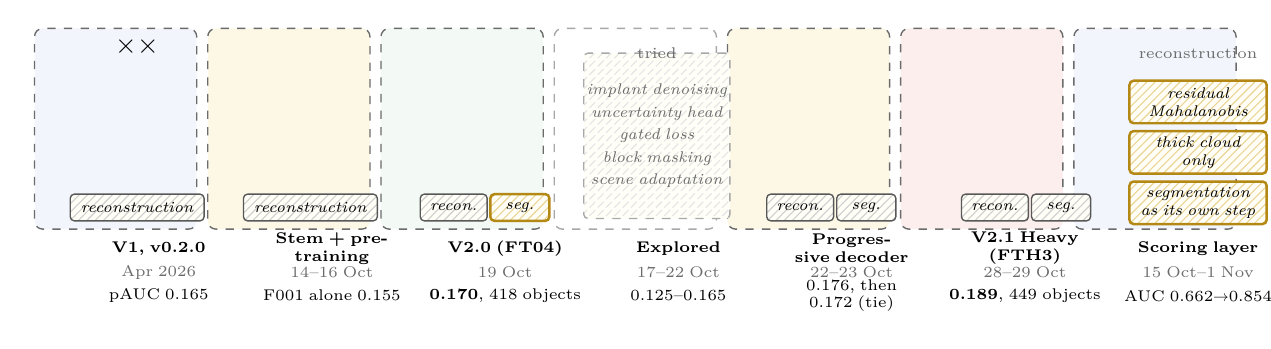
\begin{tikzpicture}[x=1mm,y=1mm,
  mb/.style={stg, pattern color=faint!55, inner sep=0.6pt, font=\itshape\fontsize{5.6}{6.4}\selectfont},
  nw/.style={stgn, inner sep=0.6pt, font=\itshape\fontsize{5.6}{6.4}\selectfont},
  ex/.style={stgx, dashed, inner sep=0.8pt, font=\itshape\fontsize{5.6}{6.4}\selectfont},
  lab/.style={font=\fontsize{5.6}{6.4}\selectfont, align=center, text width=20mm},
  ar/.style={-{Stealth[length=1mm,width=0.8mm]}, line width=0.35pt, draw=mute}]
\gen{0}{165-band grid}{mb}{1$\times$1 compressor}{mb, minimum width=10mm}{encoder}{mb}{SegFormer decoder}
\node[mb, minimum width=17mm, minimum height=3.4mm] at (0,-19.6) {reconstruction};
\gen{22}{\textcolor{ochre!80!black}{\textbf{any band list}}}{nw}{wavelength stem}{mb, minimum width=10mm}{encoder}{mb}{SegFormer decoder}
\node[mb, minimum width=17mm, minimum height=3.4mm] at (22,-19.6) {reconstruction};
\gen{44}{native bands}{mb}{wavelength stem}{mb, minimum width=10mm}{encoder}{mb}{SegFormer decoder}
\node[mb, minimum width=8.5mm, minimum height=3.4mm] at (40.2,-19.6) {recon.};
\node[nw, minimum width=7.5mm, minimum height=3.4mm] at (48.6,-19.6) {seg.};
\node[ex, text width=18mm, minimum height=21mm] at (66,-10.5) {implant denoising\\[0.6mm] uncertainty head\\[0.6mm] gated loss\\[0.6mm] block masking\\[0.6mm] scene adaptation};
\node[lab, color=mute] at (66,0) {tried};
\gen{88}{native bands}{mb}{wavelength stem}{mb, minimum width=10mm}{encoder}{nw}{progressive decoder}
\node[mb, minimum width=8.5mm, minimum height=3.4mm] at (84.2,-19.6) {recon.};
\node[mb, minimum width=7.5mm, minimum height=3.4mm] at (92.6,-19.6) {seg.};
\gen{110}{native bands}{mb}{wavelength stem, 64}{nw, minimum width=18mm}{encoder, 3$\times$ wide}{mb}{progressive decoder}
\node[mb, minimum width=8.5mm, minimum height=3.4mm] at (106.2,-19.6) {recon.};
\node[mb, minimum width=7.5mm, minimum height=3.4mm] at (114.6,-19.6) {seg.};
\node[lab, color=mute] at (132,0) {reconstruction};
\node[nw, text width=17mm, minimum height=5.4mm] at (132,-6.2) {residual\\Mahalanobis};
\node[nw, text width=17mm, minimum height=5.4mm] at (132,-12.6) {thick cloud\\only};
\node[nw, text width=17mm, minimum height=5.4mm] at (132,-19) {segmentation\\as its own step};
\foreach \x/\n/\d/\r in {
  {0/V1, v0.2.0/Apr 2026/pAUC 0.165},
  {22/Stem + pretraining/14--16 Oct/F001 alone 0.155},
  {44/V2.0 (FT04)/19 Oct/\textbf{0.170}, 418 objects},
  {66/Explored/17--22 Oct/0.125--0.165},
  {88/Progressive decoder/22--23 Oct/0.176, then 0.172 (tie)},
  {110/V2.1 Heavy (FTH3)/28--29 Oct/\textbf{0.189}, 449 objects},
  {132/Scoring layer/15 Oct--1 Nov/AUC 0.662$\to$0.854}}
  {\node[lab] at (\x,-24.8) {\textbf{\n}};
   \node[lab, color=mute] at (\x,-27.8) {\d};
   \node[lab] at (\x,-30.8) {\r};}
\begin{scope}[on background layer]
\foreach \x/\f in {0/pB,22/pY,44/pG,88/pY,110/pR,132/pB} \node[grp, fill=\f!28, minimum width=20.6mm, minimum height=25.5mm, inner sep=0] at (\x,-9.6) {};
\node[grp, draw=faint, minimum width=20.6mm, minimum height=25.5mm, inner sep=0] at (66,-9.6) {};
\end{scope}
\end{tikzpicture}}

\vspace{1mm}
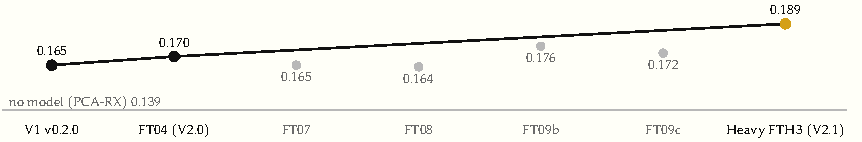
\includegraphics[width=\textwidth]{figures/chart_generations.pdf}
%% src: R p.4 Figure 3 and Table 3
\take{Shipped generations in ink, experiments that did not beat the shipped model in grey; each column adds the part outlined in ochre.}
\src{Also tried, not shipped: uncertainty head 0.125 / 0.163; per-scene adaptation 0.160. Pretrained only: 0.155 (FT04 size), 0.166 (Heavy).}
%% src: R p.4 Table 3
\end{frame}

\begin{frame}{A2 Namer runs}
\begin{columns}[T,onlytextwidth]
\column{0.54\textwidth}
\fitw{\fontsize{6.6}{7.9}\selectfont\begin{tabular}{@{}l>{\raggedright}p{24mm}>{\raggedright\arraybackslash}p{44mm}@{}}
\toprule
run & change & result\\
\midrule
N001 & linear level-1 head & level 1 at chance, 0.49--0.52 (0.50 at full fill, where ACE gets 0.87)\\
N001b & level 1 by matching & passes on all three sensors, +0.20 / +0.17 / +0.14 over ACE; \textbf{shipped}\\
N002 & textile held out & open set: 46--47\,\% of textile still called \mm{}\\
N003 & mixed spectra in a class, warped wavelengths, dropout & matched N001b on EnMAP, no gain; N001b ships\\
PV & 50 in-scene solar-panel spectra & no effect, 0.248 $\to$ 0.248\\
\bottomrule
\end{tabular}}\par
%% src: research/experiments/spectral-namer N001, N001b, N002, pv-library READMEs; R p.10 (N003), R p.15 (PV)
\vspace{1.6mm}
\kicker{N003 against the shipped N001b, EnMAP, epoch 40}\par\vspace{0.3mm}
\fitw{\fontsize{6.6}{7.9}\selectfont\begin{tabular}{@{}lrr@{}}
\toprule
measure & N001b (shipped) & N003\\
\midrule
level 1 accuracy, fill 10\,\% & 0.679 & 0.677\\
level 2 class accuracy & 0.587 & 0.588\\
\mm{} recall at ACE's false-alarm rate & 0.647 & 0.639\\
\bottomrule
\end{tabular}}\par
%% src: R p.10 Table 7
\column{0.42\textwidth}
\kicker{planted pixels from real tiles of three sensors}\par\vspace{-1.5mm}
\eqs{\[\mathbf x=\mathbf g\odot\big(a\,\mathbf t+(1-a)\,\mathbf b\big)+\mathbf n,\quad a\sim\text{log-uniform}[0.05,1]\]}
\vspace{-1.5mm}
\tx{$\mathbf t$ a library spectrum (50\,\% \mm, 25\,\% \nat, 25\,\% none), $\mathbf b$ the real background, $\mathbf g$ a smooth gain within $\pm$10\,\%, $\mathbf n$ the tile's own noise.}
\vspace{0.6mm}
\eqs{\[\mathcal L=\mathrm{BCE}(\ell,\mathrm M)+\mathrm{CE}(S_{0..6},c)+0.5\,|\hat a-a|\]}
\vspace{-1mm}
\fitw{\fontsize{6.6}{7.9}\selectfont\begin{tabular}{@{}ll@{}}
\toprule
parameters & 347,685, of which the shared stem 17,825\\
optimiser & AdamW $3\!\times\!10^{-4}$, stem at 0.3$\times$\\
run & 40 epochs $\times$ 500 steps on one H100\\
intervals & 500 resamples of 221--254 spectra per sensor\\
\bottomrule
\end{tabular}}\par
%% src: research/textbook/chapters/42-namer.tex; N001b config.json and README; R p.10 Figure 5 caption
\vspace{0.6mm}
\tx{About 34 unseen \mm{} spectra per sensor: differences much below 0.12 are not resolved.}
%% src: R p.10
\end{columns}
\end{frame}

\begin{frame}{A3 HyperSL detail}
\begin{columns}[T,onlytextwidth]
\column{0.50\textwidth}
\kicker{planted targets, 10\,\% fill, 8 choices, target's own spectrum removed}\par\vspace{0.3mm}
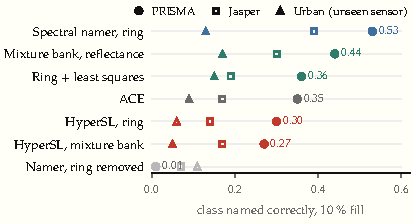
\includegraphics[width=\linewidth]{figures/chart_planted.pdf}\par
%% src: R p.14 Table 12
\tx{The background estimate matters most: ring of neighbours $>$ scene mean $>$ nothing. Without its ring the namer collapses (0.01): its call is, in effect, ``this pixel differs from its neighbours''. About 40\,\% of targets cannot be named even when pure; that caps every method near 0.6.}
%% src: R p.14
\column{0.46\textwidth}
\kicker{per-scene min-max, worked}\par\vspace{0.3mm}
\tx{Scene 1: $p_1=(0.10,0.30)$, $p_2=(0.20,0.50)$, $p_3=(0.30,0.40)$ give $p_2'=(0.5,1.0)$. The same $p_2$ in scene 2 gives $(0.43, 0.75)$. One bright anomaly moves every other pixel's input. Angle $p_2,p_3$: 15.1$^\circ$ before, 36.9$^\circ$ after.}
%% src: R p.12; docs/training/anomaly-detection/30-min-max-and-the-library.md
\vspace{1.2mm}
\kicker{the decision}\par\vspace{0.3mm}
\fitw{\fontsize{6.6}{7.9}\selectfont\begin{tabular}{@{}>{\raggedright}p{24mm}>{\raggedright}p{22mm}>{\raggedright\arraybackslash}p{22mm}@{}}
\toprule
need & HyperSL & Indradhanu\\
\midrule
same spectrum, same input & min-max per scene & fixed curve over wavelength\\
library spectra have an input & none & same stem\\
band lists with gaps & groups by band position & 40\,nm wavelength bins\\
a pixel never rebuilds itself & rebuilds from its own bands & hides whole pixels\\
cloud in pretraining & cloud-free & cloud and haze seen\\
\bottomrule
\end{tabular}}\par
%% src: R p.14 (fixes it would need)
\vspace{1mm}
\src{HyperSL ran on a 149-band PRISMA axis with its default mask ratio; nothing tuned on the bench. Subtle tier suffers most: 29.7\,\% found against 35.0\,\% with no model.}
%% src: R p.13, R p.15
\end{columns}
\end{frame}

\begin{frame}{A4 Evaluation method}
\begin{columns}[T,onlytextwidth]
\column{0.50\textwidth}
\kicker{partial AUC, the headline measure}\par\vspace{-1.5mm}
\eqs{\[\mathrm{pAUC}_m=\frac1m\int_0^m\!\mathrm{TPR}(f)\,df=\frac1P\sum_{p}\frac{\max(0,\,m-\mathrm{FPR}(p))}{m}\]}
\vspace{-1mm}
\tx{$m=0.01$; $\mathrm{FPR}(p)$ is the share of background pixels scoring at or above target pixel $p$.}
%% src: research/textbook/chapters/31-measures.tex
\vspace{1mm}
\kicker{paired object bootstrap}\par
\begin{itemize}\setlength{\itemsep}{0.3mm}\fontsize{6.6}{7.9}\selectfont
\item Resample the 909 objects with replacement, 2,000 draws; score both methods on each draw; report the 95\,\% interval of $B-A$.
\item Objects, not pixels, are the independent unit; pairing removes shared object difficulty.
\item It does not cover checkpoint-to-checkpoint variation, so three neighbouring checkpoints were checked.
\end{itemize}
%% src: R p.2 Table 2; R p.15 (bench size)
\column{0.46\textwidth}
\kicker{all measures; excl. = thick cloud left out}\par\vspace{0.3mm}
\fitw{\fontsize{6.6}{7.9}\selectfont\begin{tabular}{@{}lrrrrrr@{}}
\toprule
& \multicolumn{2}{c}{pAUC} & \multicolumn{2}{c}{top 1\,\%} & top 0.1\,\% & ROC\\
method & all & excl. & all & excl. & excl. & excl.\\
\midrule
\rowcolor{ochre!14}V2 Heavy & 0.175 & \textbf{0.189} & 422 & \textbf{449} & 16.0\,\% & 0.869\\
V2.0 (FT04)$^*$ & 0.162 & 0.170 & 415 & 418 & 15.8\,\% & 0.852\\
no model (PCA-RX) & 0.128 & 0.139 & 361 & 377 & 8.5\,\% & 0.842\\
MNF-RX & 0.075 & 0.097 & 249 & 280 & 5.2\,\% & 0.753\\
HyperSL residual & 0.083 & 0.095 & 350 & 369 & 6.7\,\% & 0.761\\
HyperSL own error & 0.018 & 0.018 & 130 & 137 & 4.3\,\% & 0.628\\
random & & & 93 & 93 & 1.1\,\% & 0.5\\
\bottomrule
\end{tabular}}\par
\src{$^*$ FT04 with its own cloud and thin-cloud mask.}
%% src: R p.6 Table 5
\vspace{1mm}
\kicker{why only thick cloud}\par\vspace{0.2mm}
\tx{Heavy's thin-cloud class fires on haze: 75.4\,\% of Set-4's pixels and 209 of its 230 targets. Cloud is out of scope; water is in, because vessels are targets.}
%% src: R p.6-7
\end{columns}
\end{frame}

\begin{frame}{A5 Deployment}
\begin{columns}[T,onlytextwidth]
\column{0.50\textwidth}
\kicker{air-gapped evaluation server}\par
\begin{itemize}\setlength{\itemsep}{0.4mm}\fontsize{6.6}{7.9}\selectfont
\item One H200 (140\,GB) with a 16-core CPU and 64\,GB RAM; no network.
\item The product (web API, worker, frontend, database) and the atmospheric-correction container arrive as offline archives with checksums; IT scans each image.
\item Update and rollback replace containers and never touch data volumes or settings; rehearsed on a simulated copy of the server.
\item Atmospheric correction runs with networking disabled, as non-root, on GPU or CPU only. DEM tiles (Copernicus 30\,m South Asia, 90\,m worldwide) are staged locally.
\end{itemize}
%% src: R p.21 (hardware); docker/airgap-update/README.md; container README; R p.19 (DEM)
\vspace{1mm}
\kicker{atmospheric-correction container}\par\vspace{0.3mm}
\fitw{\fontsize{6.6}{7.9}\selectfont\begin{tabular}{@{}ll@{}}
\toprule
core & ISOFIT 4.1.5, sRTMnet emulator, 6S compiled for x86-64-v3/v4\\
tests & 81 passed, 54\,\% coverage\\
size & 22\,GB image, 8.98\,GB compressed\\
\bottomrule
\end{tabular}}\par
%% src: container README (4.1.5, sRTMnet); R p.19 (6S -O3 x86-64-v3/v4); EXPERIMENT_LOG.md AC26-BLD (81, 54 %, 22 / 8.98 GB)
\column{0.46\textwidth}
\kicker{worker cost, one PRISMA scene, 185 bands (s)}\par\vspace{0.3mm}
\fitw{\fontsize{6.6}{7.9}\selectfont\begin{tabular}{@{}lrrrr@{}}
\toprule
& reconstruct & segment & score & total\\
\midrule
Heavy, 2 threads & 1629 & 185 & 4 & 1819\\
Heavy, 16 threads & 402 & 47 & 4 & 454\\
FT04, 16 threads & 236 & 32 & & 274\\
\bottomrule
\end{tabular}}\par
%% src: research/experiments/indradhanu-finetune/FTH3-heavy-joint-more2/README.md (worker CPU cost)
\vspace{1mm}
\kicker{superpixel size against accuracy, AVIRIS-NG window vs JPL}\par\vspace{0.3mm}
\fitw{\fontsize{6.6}{7.9}\selectfont\begin{tabular}{@{}lrrr@{}}
\toprule
superpixels, per-pixel step & time & land MAE & median angle\\
\midrule
50, analytical & 40.8 min & 0.0056 & 2.15$^\circ$\\
200, analytical & 17.8 min & 0.0056 & 2.17$^\circ$\\
200, empirical line & 11.3 min & 0.0056 & 2.17$^\circ$\\
\rowcolor{ochre!14}400, empirical line & 7.5 min & 0.0057 & 2.19$^\circ$\\
\bottomrule
\end{tabular}}\par
%% src: EXPERIMENT_LOG.md AC26-FAST; R p.18 (40.8 -> 7.5 min, 0.0056 -> 0.0057)
\vspace{0.6mm}
\tx{Before the speed work: up to 75+ min for PRISMA and EnMAP and nearly 6 h for a full AVIRIS-NG scene; 12--14\,GB scenes now fit the sub-2-hour window.}
%% src: R p.19
\end{columns}
\end{frame}

\begin{frame}{A6 HAD100}
\begin{columns}[T,onlytextwidth]
\column{0.52\textwidth}
\kicker{public benchmark, official protocol, against Li et al.\ 2023}\par\vspace{0.2mm}
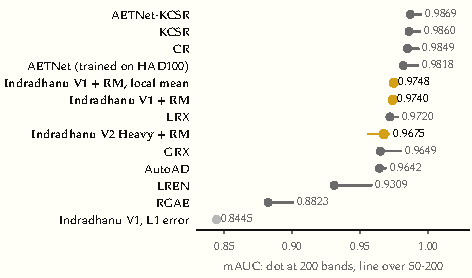
\includegraphics[width=\linewidth]{figures/chart_had100.pdf}\par
%% src: research/experiments/dual-window-mahalanobis/README.md section 4b and EXPERIMENT_LOG.md "Against the published HAD100 leaderboard" (published rows: Li et al., IEEE TGRS 2023, Table V); results/auc_summary.json had100_official_protocol
%% src: V2 Heavy rows: research/experiments/had100-v2heavy/README.md and results/mauc_summary.json (input handling A, pooled affine onto training statistics; FTH3 epoch 5 via the product inferencer + RM)
\take{At 200 bands residual Mahalanobis sits 0.013 (V1) and 0.019 (V2 Heavy) below the best, above GRX and the deep reconstruction baselines.}
\vspace{0.5mm}
\tx{On 64$\times$64 crops plain RX already scores 0.96--0.98, so HAD100 ranks methods differently from our PRISMA bench.}
\column{0.45\textwidth}
\kicker{protocol}\par\vspace{0.2mm}
\tx{100 crops of 64$\times$64 from 94 AVIRIS-NG tiles (3,567 anomaly pixels, 460 objects), L1B radiance, 276 ``good'' bands; papers then take the first 50 / 100 / 200. Measure: mAUC, the mean per-crop ROC-AUC. Our GRX reproduces the paper's GRX to four decimals.}
%% src: research/experiments/benchmarks/README.md sections 2 and 5; dual-window README 4b (calibration)
\vspace{0.6mm}
\kicker{our runs, mAUC}\par\vspace{0.2mm}
\fitw{\fontsize{6.4}{7.6}\selectfont\begin{tabular}{@{}lrrrrr@{}}
\toprule
& 50\,b & 100\,b & 200\,b & 276\,b / full & no Kakinada\\
\midrule
GRX & 0.9799 & 0.9714 & 0.9649 & 0.9634 & 0.9611\\
PCA30-RX & 0.9797 & 0.9603 & 0.9636 & 0.9648 & 0.9627\\
\rowcolor{ochre!14}Indradhanu V2 Heavy + RM & 0.9714 & 0.9559 & 0.9675 & 0.9703 & 0.9684\\
\quad local mean 5/15 & 0.9715 & 0.9565 & 0.9688 & 0.9714 & 0.9696\\
\rowcolor{ochre!14}Indradhanu V1 + RM & & & & 0.9740 & 0.9724\\
\quad local mean 5/15 & & & & 0.9748 & 0.9732\\
\bottomrule
\end{tabular}}\par
\src{V1 reads only its 165-band grid, so one value fills every column. ``No Kakinada'': 94 crops, at full bands, after removing 6 from a line flown 1--2\,km from a training swath.}
%% src: auc_summary.json (all-100 means); per-crop C:/Users/FITT/Documents/public_had_datasets/dual_window_public/had100_protocol.json (means over the 94 non-ang20180227t082814 crops; the all-100 means reproduce auc_summary exactly); benchmarks README section 3 (Kakinada, 6/100)
\vspace{0.6mm}
\tx{\textbf{Reading.} V2 Heavy ties V1 (0.970 vs 0.974 at full bands; 47/52 crops, $p=0.5$) on an airborne radiance benchmark outside its training domain (2--8\,m, US/Swiss), while reading every band count natively; V1 needs its fixed 165-band grid. V2 beats GRX and PCA30-RX at 200 and 276 bands, not at 50. The leaders are local collaborative-representation detectors; AETNet trains on HAD100's own normal tiles.}
%% src: had100-v2heavy README (47 / 52, p = 0.5; 45 / 49, p = 0.44 on 94; beats GRX/PCA30-RX at 200 and full, not 50; L1 0.860 vs 0.845; 2-8 m, North America and Switzerland)
%% src: dual-window README sections 3-4 (model v0.2.0 epoch200; transfer caveat; why leaders lead); residual-rx-2026-10-21/EXPLAINER.md line 5 (v0.2.0); no HAD100 run found under indradhanu-finetune or indradhanu-se-pretrain
\end{columns}
\end{frame}

\begin{frame}{A7 HAD100 methods on our bench}
\begin{columns}[T,onlytextwidth]
\column{0.49\textwidth}
\kicker{pAUC, FPR $\le$1\,\%, thick cloud excluded}\par\vspace{0.2mm}
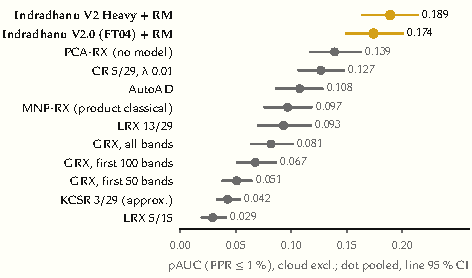
\includegraphics[width=\linewidth]{figures/chart_prisma_had100.pdf}\par
\column{0.49\textwidth}
\kicker{objects in the top 1\,\% of 909, thick cloud excluded}\par\vspace{0.2mm}
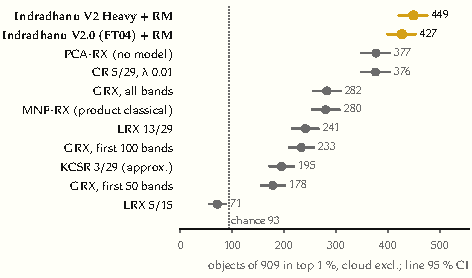
\includegraphics[width=\linewidth]{figures/chart_prisma_had100_objects.pdf}\par
\end{columns}
%% src: research/experiments/prisma-bench-had100-baselines/README.md, results.md, results.json (same evaluator; sanity: FTH3 0.1892/449, PCA-RX 0.1390/377, MNF-RX 0.0966/280 reproduced)
\vspace{1mm}
\take{None of the HAD100 methods comes close: the best, CR, reaches 0.127 against 0.189 ($-0.063$ [$-0.090$, $-0.035$]) and ties the no-model PCA-RX on objects (376 vs 377; V2 Heavy 449).}
\vspace{0.4mm}
\tx{The HAD100 ranking (KCSR $>$ CR $>$ LRX $>$ GRX) does not carry over to 30\,m PRISMA. Windows are HAD100's settings; CR's $\lambda$ was picked on the bench (optimistic); CR and KCSR run on a 30-dimensional projection keeping 99.97\,\% of the energy; KCSR approximated. AutoAD on set 1 only: 0.103 against V2 Heavy 0.262. Dot pooled over four scenes, line 95\,\% paired bootstrap.}
\end{frame}

\end{document}
